% 2> /dev/null; latexmk -pdflatex="pdflatex -synctex=1" -shell-escape  main -pdf ${0%.*} && (xdg-open ${0%.*}.pdf&); exit
%----------------------------------------------------------------------------------------
%	PACKAGES AND DOCUMENT CONFIGURATIONS
%----------------------------------------------------------------------------------------

\documentclass[11pt]{article}

% Adjusting margins to personal my need
\addtolength{\oddsidemargin}{-.75in}
\addtolength{\evensidemargin}{-.75in}
\addtolength{\textwidth}{1.5in}
\addtolength{\topmargin}{-.75in}
\addtolength{\textheight}{1.5in}

% Graphics
\usepackage{caption}
\usepackage{subcaption}
\usepackage{graphicx}
\graphicspath{{figures/}}

% Math
\usepackage{amssymb}
\usepackage{amsmath} % Required for some math elements 

% Other
\usepackage{algorithmic}
\usepackage{array}
%\usepackage{lipsum}
\usepackage{hyperref}
\usepackage[dvipsnames]{xcolor}

\usepackage{biblatex} %Imports biblatex package
\addbibresource{Tadashi_Refs.bib} %Import the bibliography file
\DeclareUnicodeCharacter{0301}{\'{e}}



%----------------------------------------------------------------------------------------
%	MAIN PART
%----------------------------------------------------------------------------------------

\begin{document}

\title{CENTER FOR NON-PERTURBATIVE STUDIES OF FUNCTIONAL MATERIALS UNDER NON-EQUILIBRIUM CONDITIONS\\Computational Materials Sciences Mid-Term Review} % Title

\date{\today} % Date for the report
\author{Hello}
% \author{
% {\bf FWP Number:}  SWC1675 &
% {\bf Lead Institution:} Lawrence Livermore National Laboratory &
% {\bf Project Director:}  Tadashi Ogitsu Ph.D. &
% {\bf Title:}  Senior Staff Scientist &
% {\bf Phone:}  (925) 422-8511 &
% {\bf Email:} ogitsu1@llnl.gov &
% {\bf Partner Institutions:} Lawrence Berkeley National Laboratory & SLAC National Accelerator Laboratory}

\maketitle % Inserts the title, author and date
{\bf\color{red}
% Notes:
\begin{itemize}
    \item Imagine your are a reviewer. Can you find the information relevant for a review criteria easily? Is your explanation clearly and effectively addressing the criteria?
    \item The Review Documents must be formatted for standard 8.5” by 11” paper with 1-inch margins on all sides and a font that is no smaller than Times New Roman 11pt. Figures, charts, tables, captions, etc., may include text smaller than these requirements as long as it is still legible without magnification.
    \item Page limits are imposed for sections 1,3-6, which will results in 20 pages total (2. budget is excluded).
    \item Each major section has to start from the top of page.
    \item Synergy is critical
    \item Mention ECN somewhere.
    \item Check if our paper submitted, type, scope and acknowledgment look good
    \item Consistency between organization chart and the others need to be checked again
\end{itemize}
}

\clearpage
%----------------------------------------------------------------------------------------
%	Table of Content
%----------------------------------------------------------------------------------------
\setcounter{tocdepth}{2}
\tableofcontents


\clearpage

%----------------------------------------------------------------------------------------
%	Main Part
%----------------------------------------------------------------------------------------
\section{Organization Chart}
\label{sec:organization}

\begin{figure}[ht]
    \centering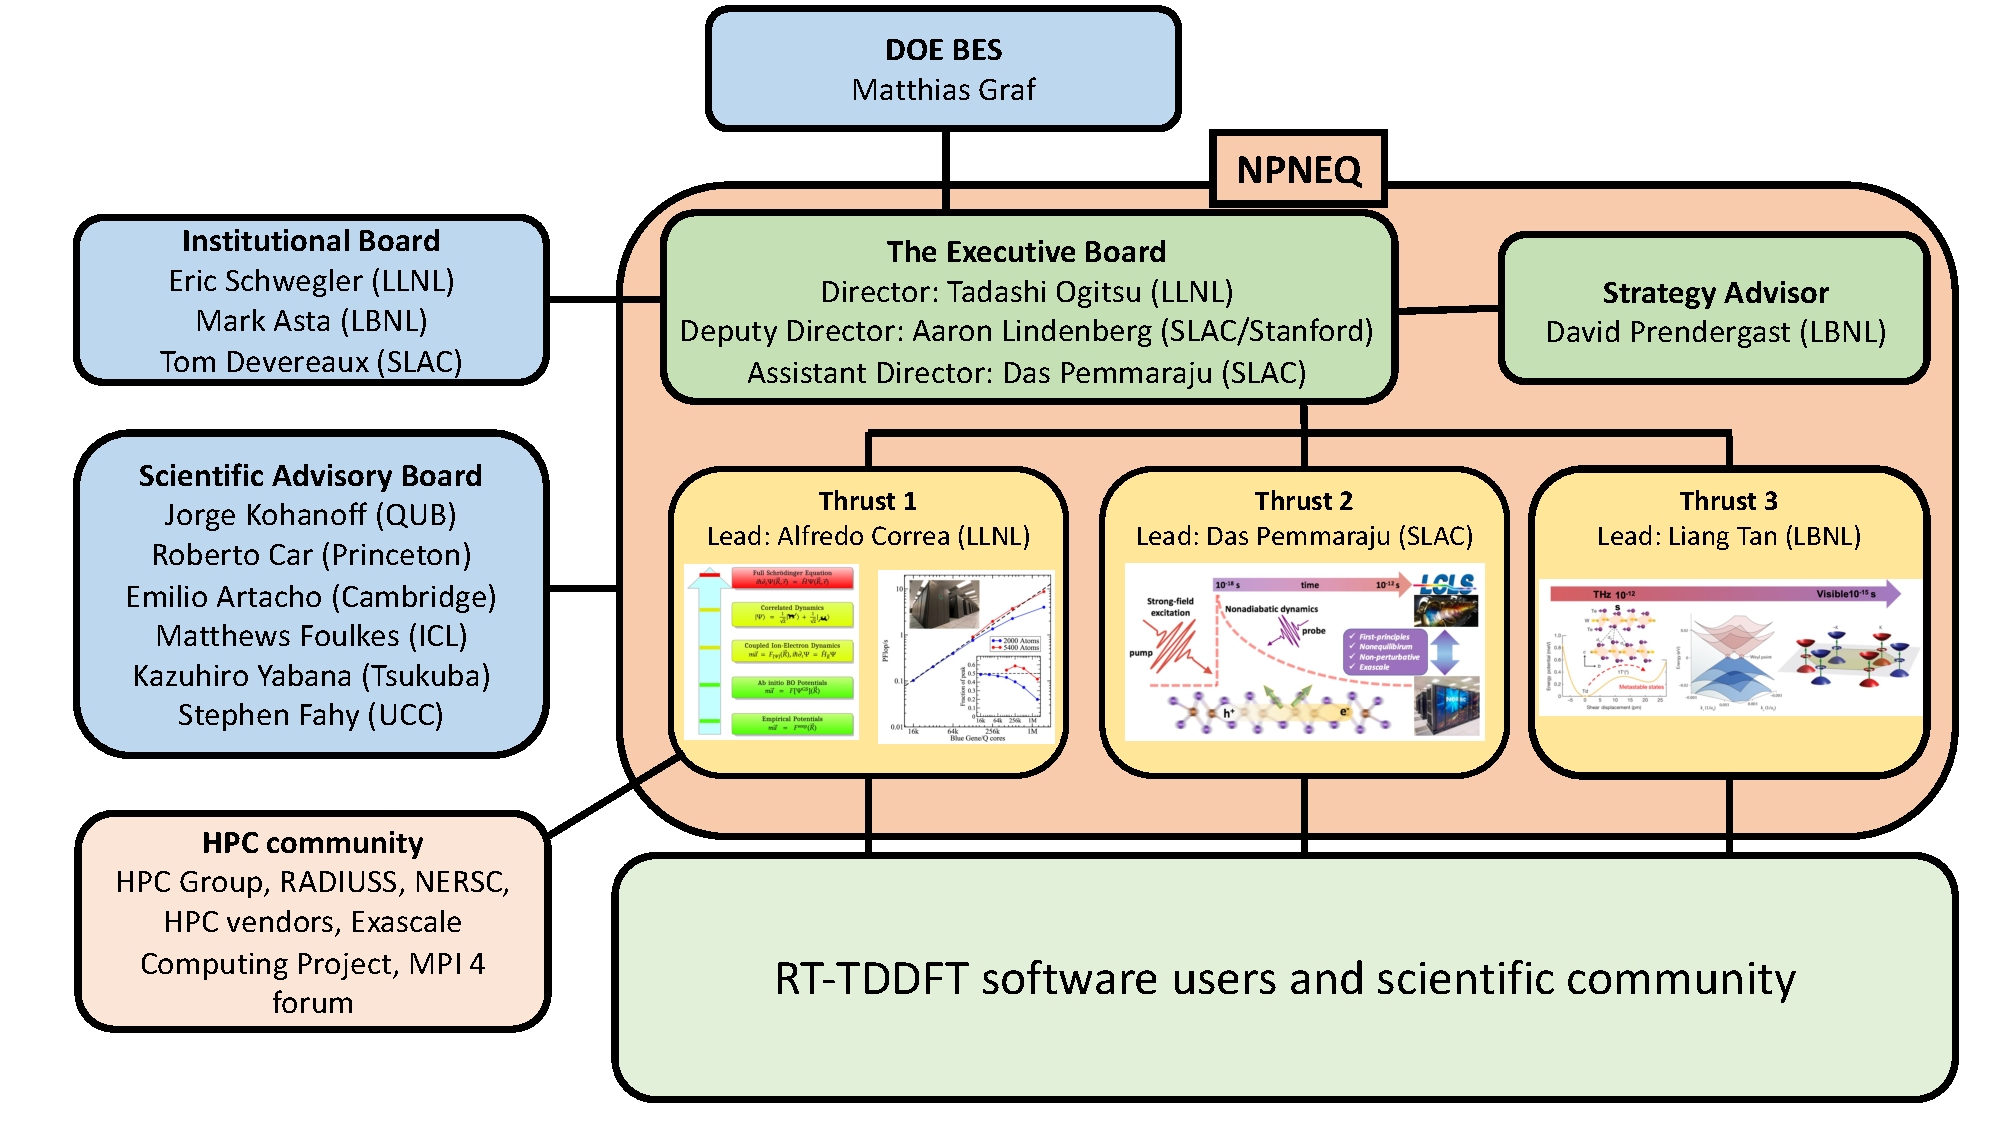
\includegraphics[width=1.0\linewidth]{figures/OrganizationalStructure.pdf}
    \caption{Organization structure of NPNEQ and its relation to DOE PM, SAB, Institutional Board, HPC community, RT-TDDFT users, and the scientific community.}
    \label{fig:organization}
\end{figure}

\clearpage


\section{Budget And Staffing Tables}
\label{sec:budget}
\begin{itemize}
    \item \textcolor{red}{Provide an update to Table 1 and Table 2 in your proposal. Table 1: Senior/Key personnel on the application and institutional affiliations and Table 2: Summary Budget information for all partner institutions. Add new Table 3: Budget by Task which summarizes the allocated/planned funding for the high-level research tasks (thrusts) by year. In the text for this section, refer readers to appendix B for additional information on staffing roles and student/postdoctoral participation.}
    \item \textcolor{red}{Review criteria for Reasonableness and Appropriateness of the Proposed Budget: Comment on the appropriateness of the proposed budget and the distribution of the funds/staffing among research tasks/themes, software development, and PIs/institution (if applicable).
}

\end{itemize}


\begin{table}[ht]
    \centering\small
    \begin{tabular}{|l|l|l|l|l|}
    \hline
        Last Name & First Name & Effort level & Role & Institution \\
        \hline
        {\bf\textcolor{purple}{Ogitsu}} & {\bf\textcolor{purple}{Tadashi}} & \bf\textcolor{purple}{0.25FTE} & \bf\textcolor{purple}{Director} & LLNL \\
        {\bf\textcolor{orange}{Correa}} & \bf\textcolor{orange}{Alfredo} & \bf\textcolor{orange}{0.5FTE} & \bf\color{orange} Software Design Lead & LLNL \\
        \color{orange}Andrade & \color{orange}Xavier & \color{orange}0.5FTE &\color{orange}Software GPU Implementation & LLNL \\ \hline
        \bf\color{red}Tan & \bf\color{red}Liang & \bf\color{red}0.04FTE & \bf\color{red} Interpretation Lead & LBNL \\
        \color{red}Rajpurohit & \color{red}Sangeeta & \color{red}1.0 PD & \color{red}Interpretation & LBNL \\
        \bf\color{pink}Prendergast & \bf\color{pink}David & \bf\color{pink}0.01FTE & \bf\color{pink}Advisor & LBNL \\ \hline
        \bf\color{blue}Pemmeraju & \bf\color{blue}S. C. Das & \bf\color{blue}0.1FTE &\bf\color{blue}Validation Simulation Lead & SLAC \\
        \color{blue}Kertzev & \color{blue}Alexey & \color{blue}0.975PD & \color{blue}Validation Simulation & SLAC\\
        \bf\color{green}Lindenberg & \bf\color{green}Aaron & \bf\color{green}0.01FTE & \bf\color{green} Validation Experiment Lead & SLAC/Stanford \\
        \color{green}Xiao & \color{green}Jun & \color{green}0.4625PD & \color{green}Validation Experiment & SLAC\\
        \hline
    \end{tabular}
    \caption{Senior/key personnel and institutional affiliation}
    \label{tab:senior_key_personnel}
\end{table}
\begin{table}[ht]
    \centering
    \begin{tabular}{|l|llll|l|}
    \hline
    Institution Name     & Year 1 & Year 2 & Year 3 & Year 4 & Total \\
    \hline
    Lawrence Livermore National Laboratory & \$575k & \$575k & \$575k & \$575k & \$2,300k \\
    Lawrence Berkeley National Laboratory & \$150k & \$150k & \$150k & \$150k & \$600k \\
    SLAC National Accelerator Laboratory & \$275k & \$275k & \$275k & \$275k & \$1,100k \\
    \hline
    Total budget & \$1,000k & \$1,000k & \$1,000k & \$1,000k & \$4,000k \\
   \hline 
    \end{tabular}
    \caption{Summary of budget information for lead institution and all partner institution}
    \label{tab:budget}
\end{table}

\begin{table}[ht]
    \centering
    \begin{tabular}{|l|llll|l|}
    \hline
        Tasks/Thrusts & Year 1 & Year 2 & Year 3 & Year 4 & Total Budget \\
        \hline
        Software development & \$575k & \$575k & \$575k & \$575k & \$2,300k \\
        Interpretation & \$150k & \$150k & \$150k & \$150k & \$600k \\
        Validation experiments/simulations & \$275k & \$275k & \$275k & \$275k & \$1,100k \\
        \hline
        Total Budget & \$1,000k & \$1,000k & \$1,000k & \$1,000k & \$4,000k \\
        \hline
    \end{tabular}
    \caption{Summary budget for allocated/planned funding for research tasks.}
    \label{tab:budget_by_task}
\end{table}
\clearpage
\section{Overview And Executive Summary Of Accomplishment}
\label{sec:overview}
{\small
\begin{itemize}
    \item \textcolor{red}{2 pages max.}
    \begin{enumerate}
        \item \textcolor{red}{Provide a concise introduction to the organization and research being pursued.}
        \item \textcolor{red}{Briefly sketch the background leading to the 2019 proposal, the gaps in scientific knowledge that the CMS research aims to fill, and the vision and strategic objectives of the project.}
        \item \textcolor{red}{Include an Executive Summary of the progress made since September 2019 toward
meeting its strategic objectives, making clear how the accomplishments described in detail in Section 6 below fit together as part of a synergistic research program.}
    \end{enumerate}
    \item \textcolor{red}{Review criteria for Scientific and/or Technical Merit of the Proposed Research:}
    \begin{itemize}
        \item \textcolor{red}{What new capability/functionality will the proposed software provide to the materials research community? How will the research plan attain the 4-year research and software/data goals?}
        \item \textcolor{red}{Comment on the novelty and scientific value of the proposed research. }
        \item \textcolor{red}{How widespread would be the interest in the software within the materials research community?}
        \item \textcolor{red}{How does the proposed work compare with other efforts in its field, both in terms of scientific and/or technical merit and originality?}
        \item \textcolor{red}{Comment on the progress and impact for the current award period.}
    \end{itemize}

\end{itemize}
}

\clearpage

The development of quantum mechanics in early 20th century lead to paradigm shift in materials science and engineering that were witnessed as, for example, invention of semiconductor devices etc. 
Emergence of Density Functional Theory (DFT) \cite{HohenbergKohn1964,KohnSham1965} together with breakthrough in algorithmic developments \cite{cooley1965,Cohen1975,Hamann1979,CarParrinello1985,Martin1988,Hamann1989,Vanderbilt1990,Payne1992,Bloechl1994,Klesse1999} and fast growing performance of computers contributed significantly to advancement of the modern electronic structure theory where the state-of-art experiments of the day such as angle resolved photo emission and parameter free DFT band structure calculations helped cross-validating theory and experiments. 
Note that DFT's great practicality, reasonable accuracy combined with affordable computational cost, was an important factor though not often credited.
Those excellent progresses in the 20th century were, however, mostly limited to properties described as the time independent quantum mechanical problems. 
Towards the end of century, time dependent version of DFT (TDDFT) emerged \cite{RungeGross1984} together with the progress in ultrafast experimental techniques as well as the dramatic advancement in high performance computing (HPC) driven by the architectural transition into massive parallel GPU computing.
Thanks to that, we are now positioned to probe into phenomena that are described by time dependent version of Schr\"{o}dinger equation, where spin, electronic, and ionic degree of freedoms evolve in a coupled manner.

It is in this context that DOE CMS Software Center for Nonperturbative Studies of Functional Materials under Nonequilibrium Conditions (NPNEQ) was launched in September 2019 with the initial goal of developing and distributing Open Source real-time TDDFT (RT-TDDFT) software \emph{optimized for the current and future DOE Leadership Class HPC systems} such as 
	Sierra (LLNL: 125 petaflops, active from 2018), 
	El Capitan (LLNL: 1.5 exaflops, 2023), 
	Perlmutter (NERSC: 64 petaflops, phase I active from June 2021), 
	Summit (200 petaflops, active from 2018), 
	Frontier (ORNL, 1.5 exaflops, 2023), 
	and Aurora (ANL, 1 exaflops, 2021). 

As of June 2021, the RT-TDDFT software named INQ, whose basic functions are necessary for calculating ground state electronic structure as well as its time propagation have been successfully implemented. 
Rigorous tests for scientific research such as reproducibility of relevant physical quantities have been being performed based on comparisons with well established DFT (Quantum Espresso/Qbox) and TDDFT (Octopus/Qb@ll) codes. 
GPU optimization has been successfully performed together with MPI parallel implementation, where software design ({\bf Correa}), development ({\bf Andrade}) and testing ({\bf Pemmaraju}) effort were closely coordinated with the PI {\bf Ogitsu}'s oversight, fully leveraging extensive online meetings (two 2-hour meetings per week). 
\emph{
	We have successfully executed our software development plan: INQ has now achieved excellent parallel performance using multiple GPUs with a standard DFT (GGA) based on band parallelization scheme. 
	The comprehensive report about the INQ code and its future extension plan has been summarized and submitted to a peer-reviewed journal. \cite{andrade2021inq}
}

Currently existing GPU-ready (TD)DFT codes are mostly focused on delivering GPU parallel performance only for specific types of simulations such as, hybrid exchange-correlation (BigDFT) \cite{BigDFT2018} and GW calculations (VASP),\cite{vasp2012,vasp2012b,vasp2018,vasp2019} CCSD (NWChem),\cite{NWChem2013} which have intrinsically high arithmetic intensity, or k-point parallelization (QE)\cite{QE2017,QE2020} that requires less MPI communication compared to band/grid parallelization. 
Note that (TD)DFT simulation of realistic system often requires large systems in order to take relevant factors, such as defects and interface, to material property (or device performance), and in this case, band and grid parallel become more important than k-point parallel in minimizing time to solution. 
At the time of writing this report, only real space (TD)DFT codes\cite{andrade2012time,andrade2013real,SparcX2021} in GGA level simulations are able to take advantage of the computing power of GPU suggesting that lack of interconnect bandwidth may be the root of above observation since parallel 3D-FFT is known to demand high memory and interconnect bandwidths.\cite{heFFTe2020}

Our software development strategy is comprehensive and aims to facilitate advancement of theory by highly programmable design so as a scientist who is not an expert programmer to be able to implement newly developed theory/algorithm into INQ at ease, which will help expanding the user community while extending the functionality of INQ available to scientific community. 
Through extensive communications with both scientific and HPC communities suggested that basic design of code needs to have significant flexibility in adopting code design to rapidly evolving the HPC system architecture and as the theory of RT-TDDFT. 

An important HPC example is intimately related to the critical issue of non uniform memory access (NUMA) and quickly developing a solution. 
The current challenge in parallel GPU optimization is that the code design needs to take redundant memory architecture with extremely uneven computational powers (\(\mathrm{GPU} >> \mathrm{CPU}\)), which in turn requires redundant interconnect architecture, explicitly into consideration.
In short, all the data need to be on the fast GPU in order to exploit the power of GPU and avoid additional CPU-GPU communication overhead.
We note that the cost of interconnect occupies significant portion of the total cost of a HPC system, therefore, the dual interconnect architecture is not ideal from the viewpoint of cost per performance.

In considering future plan, we must note that the issue is well recognized by the HPC community and industry, and the solutions are coming. 
For example, Apple M1 chip based on ARM architecture takes system on chip approach where a set of memory together with CPU and GPU are integrated on one chip. 
A HPC system based on such a unique memory architecture can eliminate the redundant interconnect as is seen in the current world fastest supercomputer, Fugaku. 
A64FX chip used in Fugaku is based on ARM architecture with an extension called scalable vector extension (SVE), whose modified version is now implemented in ARMv9 instruction set as SVE2. NVIDIA is currently in the process of acquiring ARM company strongly suggesting a significant change in the architecture of DOE Leadership Class HPC systems in the next several years.

The anticipated change of the HPC system architecture combined with expected growth in number of contributors who are not expert programmers made us the following choice. 
While our software development platform github/gitlab offers an elaborate functionality for developing and testing software, the workflow is specific to the software so that it has to be drafted by the software developers. 
Accordingly, we are developing a workflow specific to the INQ code including automated tests performed over multiple HPC systems, which is described in a document accessible through the repository. 
In addition, the guides for users and developers of INQ software will be published, which will take feedback from users and SABs into consideration. 
These will be critical factors for an open source software development project like ours whose value have to be shared among of all the stake holders such as researchers in scientific and HPC communities, and HPC industry.

While the software development and validation tasks were being executed, the rest of team members were tasked for experiments ({\bf Lindenberg}) and interpretation ({\bf Tan} and {\bf Prendergast}) prepared for the collaborative research projects for the second half of our funding period that take full advantage of INQ code and ultrafast experimental capability, which would play the role of ultimate validation through scientific researches that involves phenomena intimately related to coupled quantum dynamics in nonperturbative limit. 
Coordination in those efforts including INQ software development were performed through communication during all hands meetings held roughly every 6 weeks and a separate monthly meeting focusing more technical issues.

Details on the research and further software development plans, the results of our efforts during the first two years including the one that made a crucial contribution to our future research plans, the tight-binding model for coupled spin-electron-ion quantum dynamics developed by our PD, {\bf Rajuprohit}, under the supervision of {\bf Tan}, software dissemination and outreach plans are described in the next section.
 
\clearpage

\textcolor{red}{below should be in the next section perhaps}

Understanding the concept of computational intensity is crucial in designing HPC software and hardware. 
Software with a given algorithm will show a certain ratio of number of floating point operation per machine cycle/number of data copy between memory and register per machine cycle/number of data copy between (MPI) processes per machine cycle, though it may vary slightly depending on some indirect factors.
By comparing these ratios between a given simulation against that of hardware (floating point operation count, memory bandwidth, interconnect bandwidth), one can understand approximate upper limit of software performance. 
In order to understand the performance behavior of parallel GPU (TD)DFT software on a few target HPC systems, Ogitsu is currently in communication with Prof. Stanimire Tomov of U. Tennesee, whose team developed GPU ready parallel 3D-FFT library named heFFTe, which is optimized for Summit at ORNL. 
As it is known, computationally expensive parts of a GGA/LDA level DFT simulation based on planewave pseudopotential algorithm are orthonormalization of wavefunction, 3D-FFT, and non-local pseudopotential. 
Accordingly, the performance of 3D-FFT often becomes a good predictor of overall performance.

\clearpage


\section{Description Of Research Tasks, Progress, And Plans}
\label{sec:research}

{\small\color{red}
\begin{itemize}
\item 12 pages max
    \item Include an Executive Summary of the progress made since September 2019 toward
meeting its strategic objectives, making clear how the accomplishments described in detail in Section 6 below fit together as part of a synergistic research program.
\begin{enumerate}
    \item Specific research objectives associated with each task
    \item Research progress for each task since the start of the project
    \item Integration of research activities across tasks
    \item Research planned for the balance of the award period (through September 2023).
\end{enumerate}
\item In the descriptions of the tasks and their integration, the need for a collaborative, synergistic approach involving several investigators should be clearly established. The role and intellectual contribution of each senior investigator should be clear to the reviewer, and the availability of the resources necessary to accomplish the research objectives should be evident. Approximately 70\% of this section should be dedicated to research progress to date and 30\% to planned research.
    \item \textcolor{red}{Review criteria for Scientific and/or Technical Merit of the Proposed Research:}
    \begin{itemize}
        \item \textcolor{red}{What new capability/functionality will the proposed software provide to the materials research community? How will the research plan attain the 4-year research and software/data goals?}
        \item \textcolor{red}{Comment on the novelty and scientific value of the proposed research. }
        \item \textcolor{red}{How widespread would be the interest in the software within the materials research community?}
        \item \textcolor{red}{How does the proposed work compare with other efforts in its field, both in terms of scientific and/or technical merit and originality?}
        \item \textcolor{red}{Comment on the progress and impact for the current award period.}
    \end{itemize}

\end{itemize}
}
{\color{green}
Note to ourselves:
\begin{itemize}
    \item TB-INQ integration in future: forced oscillation? any idea? Keep in mind: non perturbative aspect is very important.
    \item k-points and non-orthgonal cell
    \item User defined operation for external collaborator? How to balance with performance?
    \item How to expand user base need to be spelled out: Online tutorial by Xavier in late summer, ESW, TMF users meeting (Liang gave us material), SLAC (name?) workshop, US-Africa collaboration (?)
    \item CCMS to expand collaboration: two summer student from Andre and ? with Alfredo and Kejun from Yuan with Tadashi. Perhaps, get theirs support information and relevant research area to make it more convincing and compelling.
\end{itemize}

}
\clearpage

\section{Progress and Accomplishments to date}

As outlined above, the primary strategic objective of the NPNEQ CMS center during the first 18 months of the funding period was the development of a \textbf{portable}, \textbf{extensible}, \textbf{scalable} and \textbf{reliable} DFT/RT-TDDFT framework that is fully compatible with existing petascale and near-term exascale \textbf{hybrid CPU-GPU} architectures.
This objective was achieved with the recent release of \textsc{inq}~\cite{Andrade2021}. 
In parallel however, the team also pursued multi-institutional collaborative research efforts leading to science outcomes in the area of \emph{ultrafast materials science} using alternate tools and methodologies, some of which will be incorporated into the larger INQ ecosystem of codes in future. 
In the following we provide a summary of both the software development and scientific research efforts within NPNEQ.

\subsection{Code Development}

\subsubsection{The INQ DFT/TDDFT platform} 

With the widespread adoption of Graphical Processing Units (GPUs) as a powerful and energy efficient hardware paradigm for scientific computing over the past fifteen years and with the ongoing migration of DOE's national super-computing facilities from CPU to networked hybrid CPU-GPU architectures, it is of paramount importance within computational materials science that the community has access to electronic structure codes that are fully compatible with the emerging GPU computing landscape.
The INQ platform~\cite{Andrade2021} under development by the NPNEQ team addresses this need within the context of Density Functional Theory (DFT) based approaches to materials simulation while further specializing to nonperturbative simulations of materials under nonequilibrum conditions.
During the first 18 months of this funding period, the NPNEQ center accomplished the design and development tasks necessary to deliver a modular and extensible GPU-accelerated software solution for DFT/TDDFT led by LLNL PIs \textbf{Andrade} and \textbf{Correa}.
In the following we outline the unique design features of INQ as well as it's current capabilities:

\paragraph{General features and design:}
The design philosophy of INQ differs in many important respects from established Fortran/C based DFT/TDDFT codes developed in previous decades to run on CPUs: Unlike the CPU computing model that matured decades ago, GPU computing is still rapidly evolving with different hardware designs competing for primacy in the super-computing space and vendors making significant low-level updates and optimizations on a regular basis.
\textsc{Inq} is therefore designed from the outset to be easily modified and improved on top of evolving hardware, while providing consistent results and behavior independent of specific vendor platforms. 
\textsc{Inq} achieves this goal through abstractions enabled by modern C++ programming, by implementing a clear separation between different classes of software components, namely: application (DFT/TDDFT) specific code, infrastructure (basis-set, boundary conditions, data-structures etc) code and low-level numerical library (blas, FFTs etc) code. 
\newline 
\newline
As shown in Fig.~\ref{fig:inq_design}(a), in traditional DFT/TDDFT programs, the different software components are rather tightly coupled into monolithic software units and the programmer may encounter all classes of code within a given subroutine or function. 
\textsc{Inq} on the other hand implements a hierarchical structure with an application (DFT/TDDFT) code layer that sits on top of an infrastructure library layer which gracefully handles all hardware-dependent decisions. 
A programmer working with the DFT/TDDFT layer then encounters a much simplified programming interface that syntactically resembles the relevant physics equations~(see Ref.~\cite{Andrade2021}) and is shielded from lower level representation-specific and hardware-specific details. 
This hierarchical design is critical for developing code that is hardware portable while simultaneously reducing the learning curve for new developers from the DFT community to be able to quickly add functionality in the application layer. 
Note that while interpreted scripting languages such as Python, MATLAB, etc. can provide a similar type of abstraction, there is a performance cost associated with them which is not incurred by \textsc{inq} as it relies on compiled C++.

\begin{figure}[h]
	\centering
	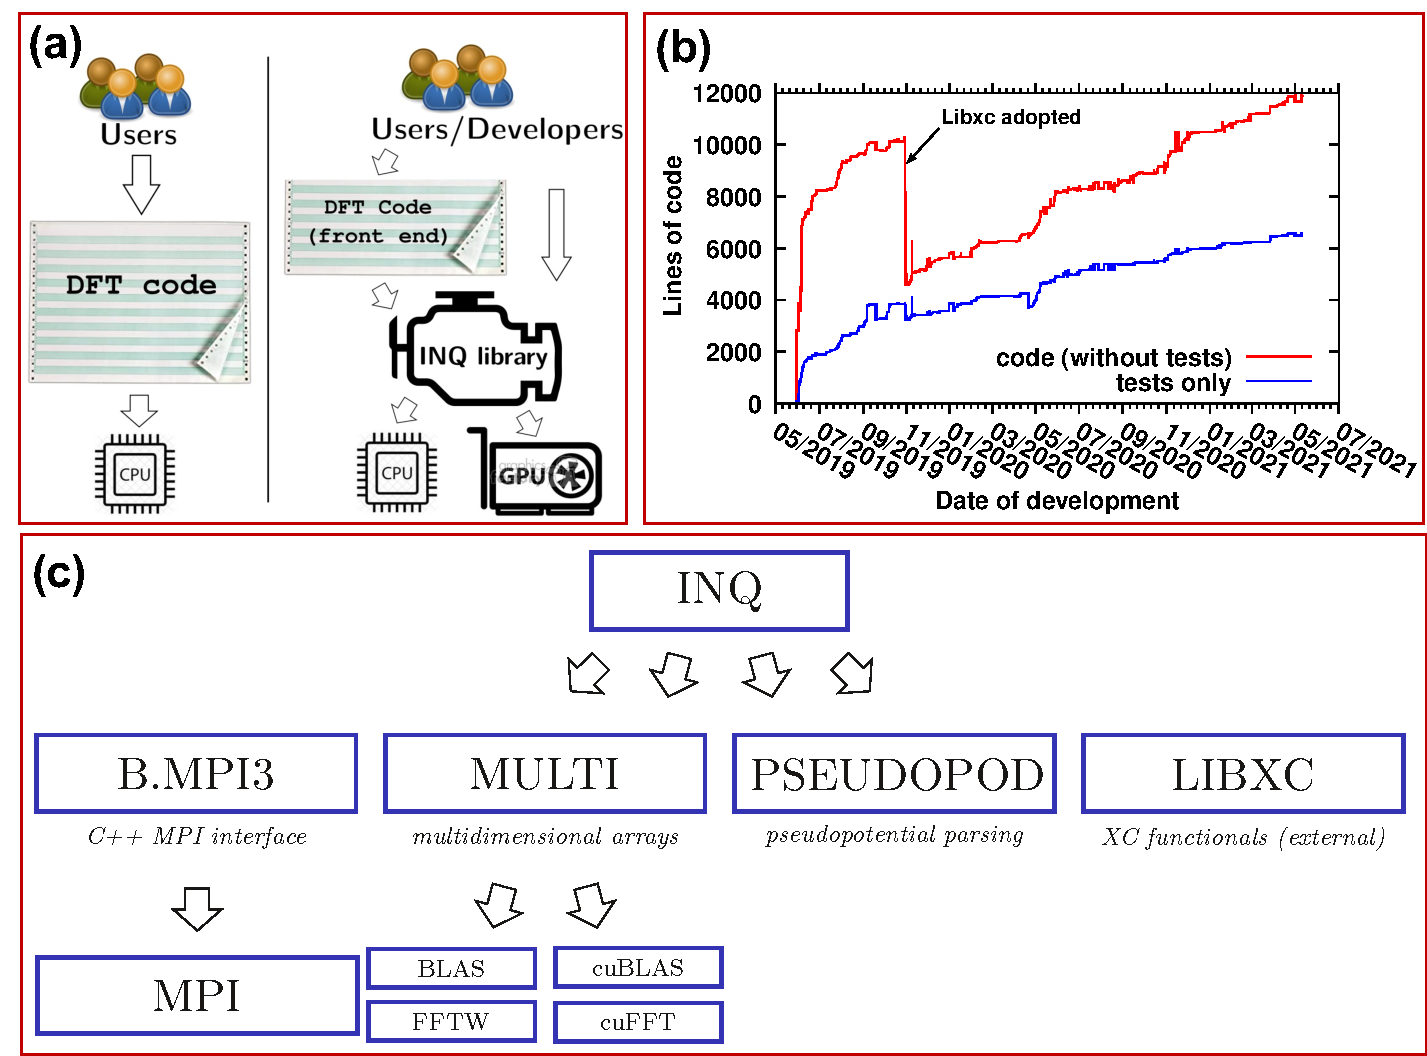
\includegraphics[width=1.0\linewidth]{figures/INQ_design_features.pdf}
	\caption{
		Key design features of the INQ framework.
		(a) INQ was built from the outset as a library that can operate on both CPU and GPU hardware,
		(b) At roughly 12,000 lines of code, INQ is extremely lightweight compared to other DFT/TDDFT codes offering comparable functionality.
		Adopting GPU-compatible \textsc{libxc} substantially reduced the size of INQ's internal codebase.
		(c) INQ brings together a highly modular hierarchy of libraries ensuring maximum adaptability with respect to future hardware and software changes.
	}
	\label{fig:inq_design}
\end{figure}

The hardware portability of \textsc{inq} is achieved in practice through a highly modular design of its library layer which brings together a number of different components that were developed both at LLNL and by the extended DFT community. 

Some of the key libraries used in INQ are:
\begin{itemize}
	\item \textbf{MULTI:} Developed by PI \textbf{Correa} at LLNL, \textsc{MULTI} provides multidimensional array access on both CPU and GPU memory models while abstracting operations over arrays without compromising maximum performance. 
	It also provides the interface between \textsc{inq} and vendor provided linear algebra, FFT and C++ standard libraries.
	\item \textbf{B.MPI3:} B-MPI3 is a C++ library wrapper for version 3.1 of the Message Passing Interface (MPI) standard that simplifies the its utilization while maintaining a similar level of performance as the more cumbersome native MPI C-language interface. 
	B.MPI3 was developed by PI \textbf{Correa} at LLNL.
	\item \textbf{PSEUDOPOD:} \textsc{PSEUDOPOD} is a CPU+GPU compatible library that handles pseudopotential (PP) parsing, filtering and other auxiliary tasks while supporting many popular PP formats as well standardized PP sets such as Pseudodojo and SG15. 
	\textsc{PSEUDOPOD} developed by PI \textbf{Andrade} at LLNL, moves PP handling from the application layer to the library layer of INQ.
	\item \textbf{LIBXC:} Libxc is a standalone library of exchange and correlation (XC) functionals initially developed by M. Marques. 
	As part of the development on \textsc{inq}, PI \textbf{Andrade} implemented a GPU extension of \textsc{libxc} that relies on cuda ‘unified memory’ to store its internal data structures. 
	\textsc{INQ} therefore has the ability to evaluate XC functionals on GPUs, which is critical to maintain all data in the GPU.
\end{itemize}

Figure~\ref{fig:inq_design}(c) shows the interaction between these \textsc{inq} modules and lower-level vendor provided libraries. 
The modularization of \textsc{inq}'s library layer affords several advantages: For instance, different components can be developed and tested independently as well as shared with other codes, to avoid duplication of work and enable collaborative development. 
Following changes to low-level hardware-optimized libraries, only a small portion of the code needs to be updated in a way that is transparent to application layer developers. 
Furthermore, by creating libraries and offloading tasks to them whenever possible, the codebase internal to \textsc{inq} can be kept relatively small as shown in Fig.~\ref{fig:inq_design}(b). 

Finally, in order to ensure reliability within a collaborative environment, \textsc{inq} adopts a test-driven development (TDD) approach in line with modern software development best practices. 
Therefore the \textsc{inq} codebase consists of both unit and functional tests that are run regularly within an automated continuous delivery platform hosted on gitlab. This workflow ensures that only code modifications that do not lead to errors anywhere in the codebase are accepted.

The result is a fully functional yet light-weight DFT/TDDFT framework that is portable across hardware platforms, offers optimal scaling on distributed hybrid CPU-GPU platforms combined with reliable numerical accuracy. 
\textsc{Inq}'s DFT/TDDFT application layer currently implements semi-local DFT total energies, forces and real-time propagation of the time-dependent KS equations within the adiabatic XC approximations for both molecular and solid-state systems within a periodic supercell framework. 
In the following, we discuss performance and validation tests of these capabilities within \textsc{inq}. 

\paragraph{GPU-MPI functionality and scaling:}
1-1.5 pages including figures

\paragraph{Validation of results:}
\begin{figure}[h]
	\centering
	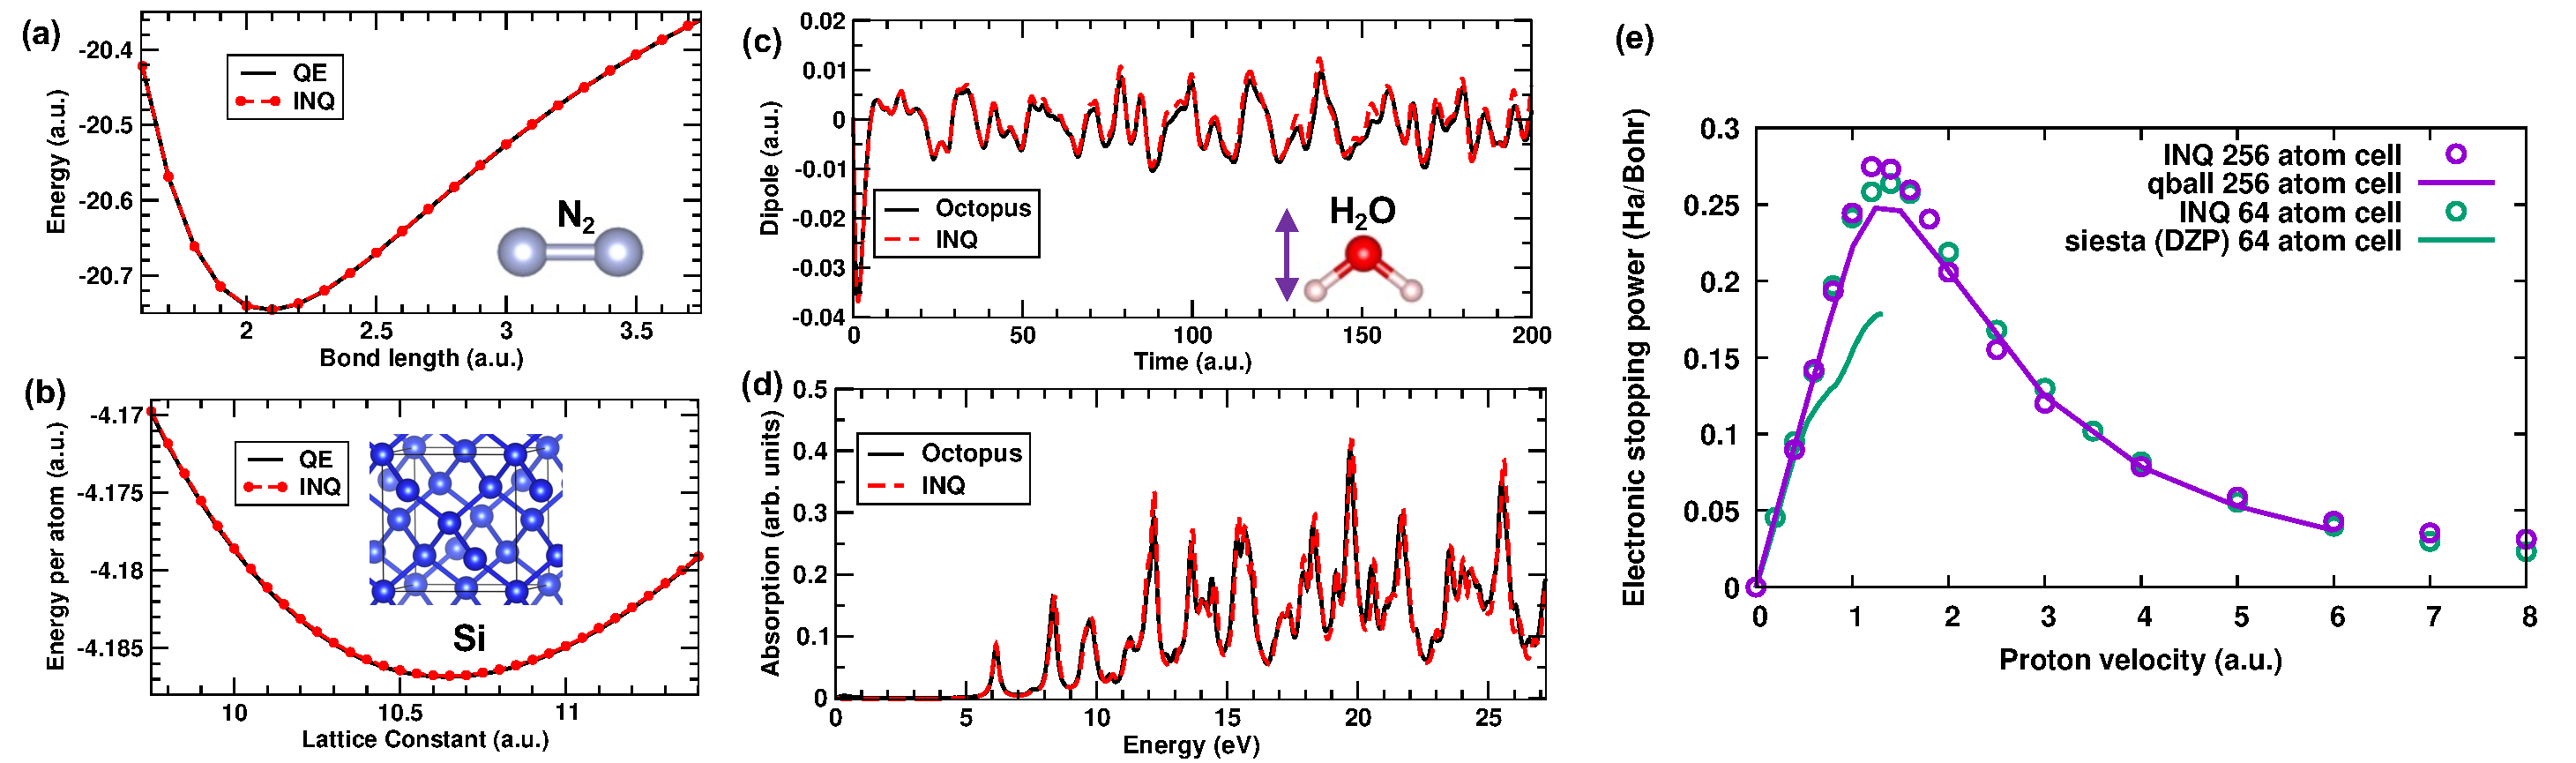
\includegraphics[width=1.0\linewidth]{figures/Results-Fig.pdf}
	\caption{
		(Adapted from Ref.~\cite{Andrade2021}.) 
		Comparison between \textsc{inq} and the established electronic structure codes \textsc{Quantum Espresso} (QE) and \textsc{octopus}.
Results for ground state total energies and real-time TDDFT optical response are shown. 
		(a) Total energy vs bond length in \(\mathrm{N_2}\).
		(b) Total energy vs lattice constant in bulk Silicon. 
		(c) Time evolution of the dipole moment in gas phase \(\mathrm{H_2O}\) following a ``kick'' perturbation. 
		(d) Linear optical absorption of molecular \(H_2O\). 
		In all cases there is a high-level of agreement between the codes.
	}
	\label{fig:inq_results}
\end{figure}

For a new scientific code it is fundamental to produce results that are consistent with other approaches and codes. 
As \textsc{inq} follows a test-driven development approach, \textsc{inq}'s codebase is continuously tested and validated at multiple levels against analytical results or benchmark data obtained from other established codes such as \textsc{Quantum Espresso}. 
We recently carried out higher level end-to-end tests of \textsc{inq} as a part of the software release validating \textsc{inq} results against corresponding quantities obtained from established plane-wave and realspace grid codes: \textsc{Quantum Espresso} (QE) and \textsc{Octopus}. 
For this purpose we chose observables such as molecular bond lengths and crystal lattice parameters based on total-energy minimization, as well as linear optical response from real-time propagation as the relevant quantities to be compared. 
For details on calculation parameters please refer to Ref.~\cite{Andrade2021}. 
As apparent from the comparisons shown in Figure~\ref{fig:inq_results}, we find that absolute total energies from \textsc{inq} are within \(0.3~\mathrm{mHartree/atom}\) of the QE reference. 
Furthermore, the optical response of a gas phase water molecule as obtained from \textsc{inq} is seen to be in excellent agreement with the corresponding result from \textsc{octopus} in the time domain (Fig.~\ref{fig:inq_results}(c)) and therefore excitation frequ1encies in the optical absorption spectrum are also found to match closely across a wide energy range. 

\textbf{Mention stopping, hook to Future work}

\subsubsection{Tight Binding model for nonequilibrium dynamics}\label{sec:tight-binding}
Within NPNEQ, \textit{ab initio} code development efforts lead by the LLNL and SLAC teams are complemented by efforts at LBNL to develop tight-binding models for non-equilibrium dynamics with the recognition that feedback between qualitative models and quantitative simulations is broadly beneficial for knowledge generation within materials science. In particular, careful model building based on first-principles calculations combined with large-scale model simulations is a promising route to produce interesting insights into the dynamic behavior of  materials driven far from equilibrium. We have developed an atomic-orbital-based tight-binding code for simulations on large time and length scales to supplement the capabilities of \textsc{inq}. These models treat
charge, spin, orbital, and atomic degrees of freedom explicitly, capturing the quantum effects of charge carriers, the non-collinear spin dynamics, and the cooperative lattice vibrations. 

With the current tight-binding code, structural and electronic optimization
can be performed to study ground state properties. 
For simulating relaxation dynamics of excited solids, 
the code supports Ehrenfest dynamics and Car-Parrinello dynamics. 
The effect of linearly polarized light field is implemented 
via the Peierls substitution method. Our recently published work
on manganites~\cite{Sangeeta2020a} demonstrates the potential of such tight-binding
models to study non-equilibrium dynamics in functional quantum materials. 

During the project period, the code has been extended to simulate multilayer
oxide structures, layered transition metal dichalcogenides (TMDC), and circularly polarized excitations. This has led to multiple scientific outputs and insights both through intra-NPNEQ ~\textcolor{red}{~\textbf{PROVIDE CITATION}} and external collaborations~\textcolor{red}{~\textbf{PROVIDE CITATION}} as outlined in the next subsection. Work is in progress to implement further extensions such as spin-orbit couplings,  van der Waals (vdW) interactions, and Nose-Hover thermostat to incorporate finite-temperature effects. Additionally, the inclusion of external magnetic fields will allow for the simulation of magnetic
excitations and magnon dispersion. Solving for these spin-waves will be done in large unit cells using
an effective spin Hamiltonian consisting of Zeeman effects, exchange interactions and magnetic
anisotropies. 



\subsection{Collaborative science}
\textcolor{red}{Descriptions of type-A projects.}

\subsubsection{Role of nonequilibrium spin-phonon coupling in enhancing bulk photovoltaic effect }\label{sec:BPVE}
During the project period, our work on the materials system of \(\mathrm{Pr_xCa_{1-x}MnO_3}\) has resulted in the discovery of a new way to enhance the bulk photovoltaic effect by optically induced phase transitions. 
These results, currently under review, are reported in the preprint Ref.~\cite{Rajpurohit2021}. 
Our study provides a unified picture of the photocurrent generation and its evolution through real-time simulations, and will have a significant impact in field of the bulk photovoltaic effect (BPVE) where understanding, predicting, and ultimately controlling the photovoltaic behavior remains a challenge.
We show theoretically that this strongly correlated oxide perovskite displays strong photocurrent enhancement when it is driven into a hidden magnetic phase transition.
This phenomenon is highly non-perturbative, and lies outside the perturbative paradigm of shift and ballistic currents used in this field. 
The maximum photoresponsivity obtained is almost an order of magnitude higher than that reported for other transition metal oxides such as \(\mathrm{BiFeO_3}\) and \(\mathrm{BaTiO_3}\).

\begin{figure}[ht]
    \centering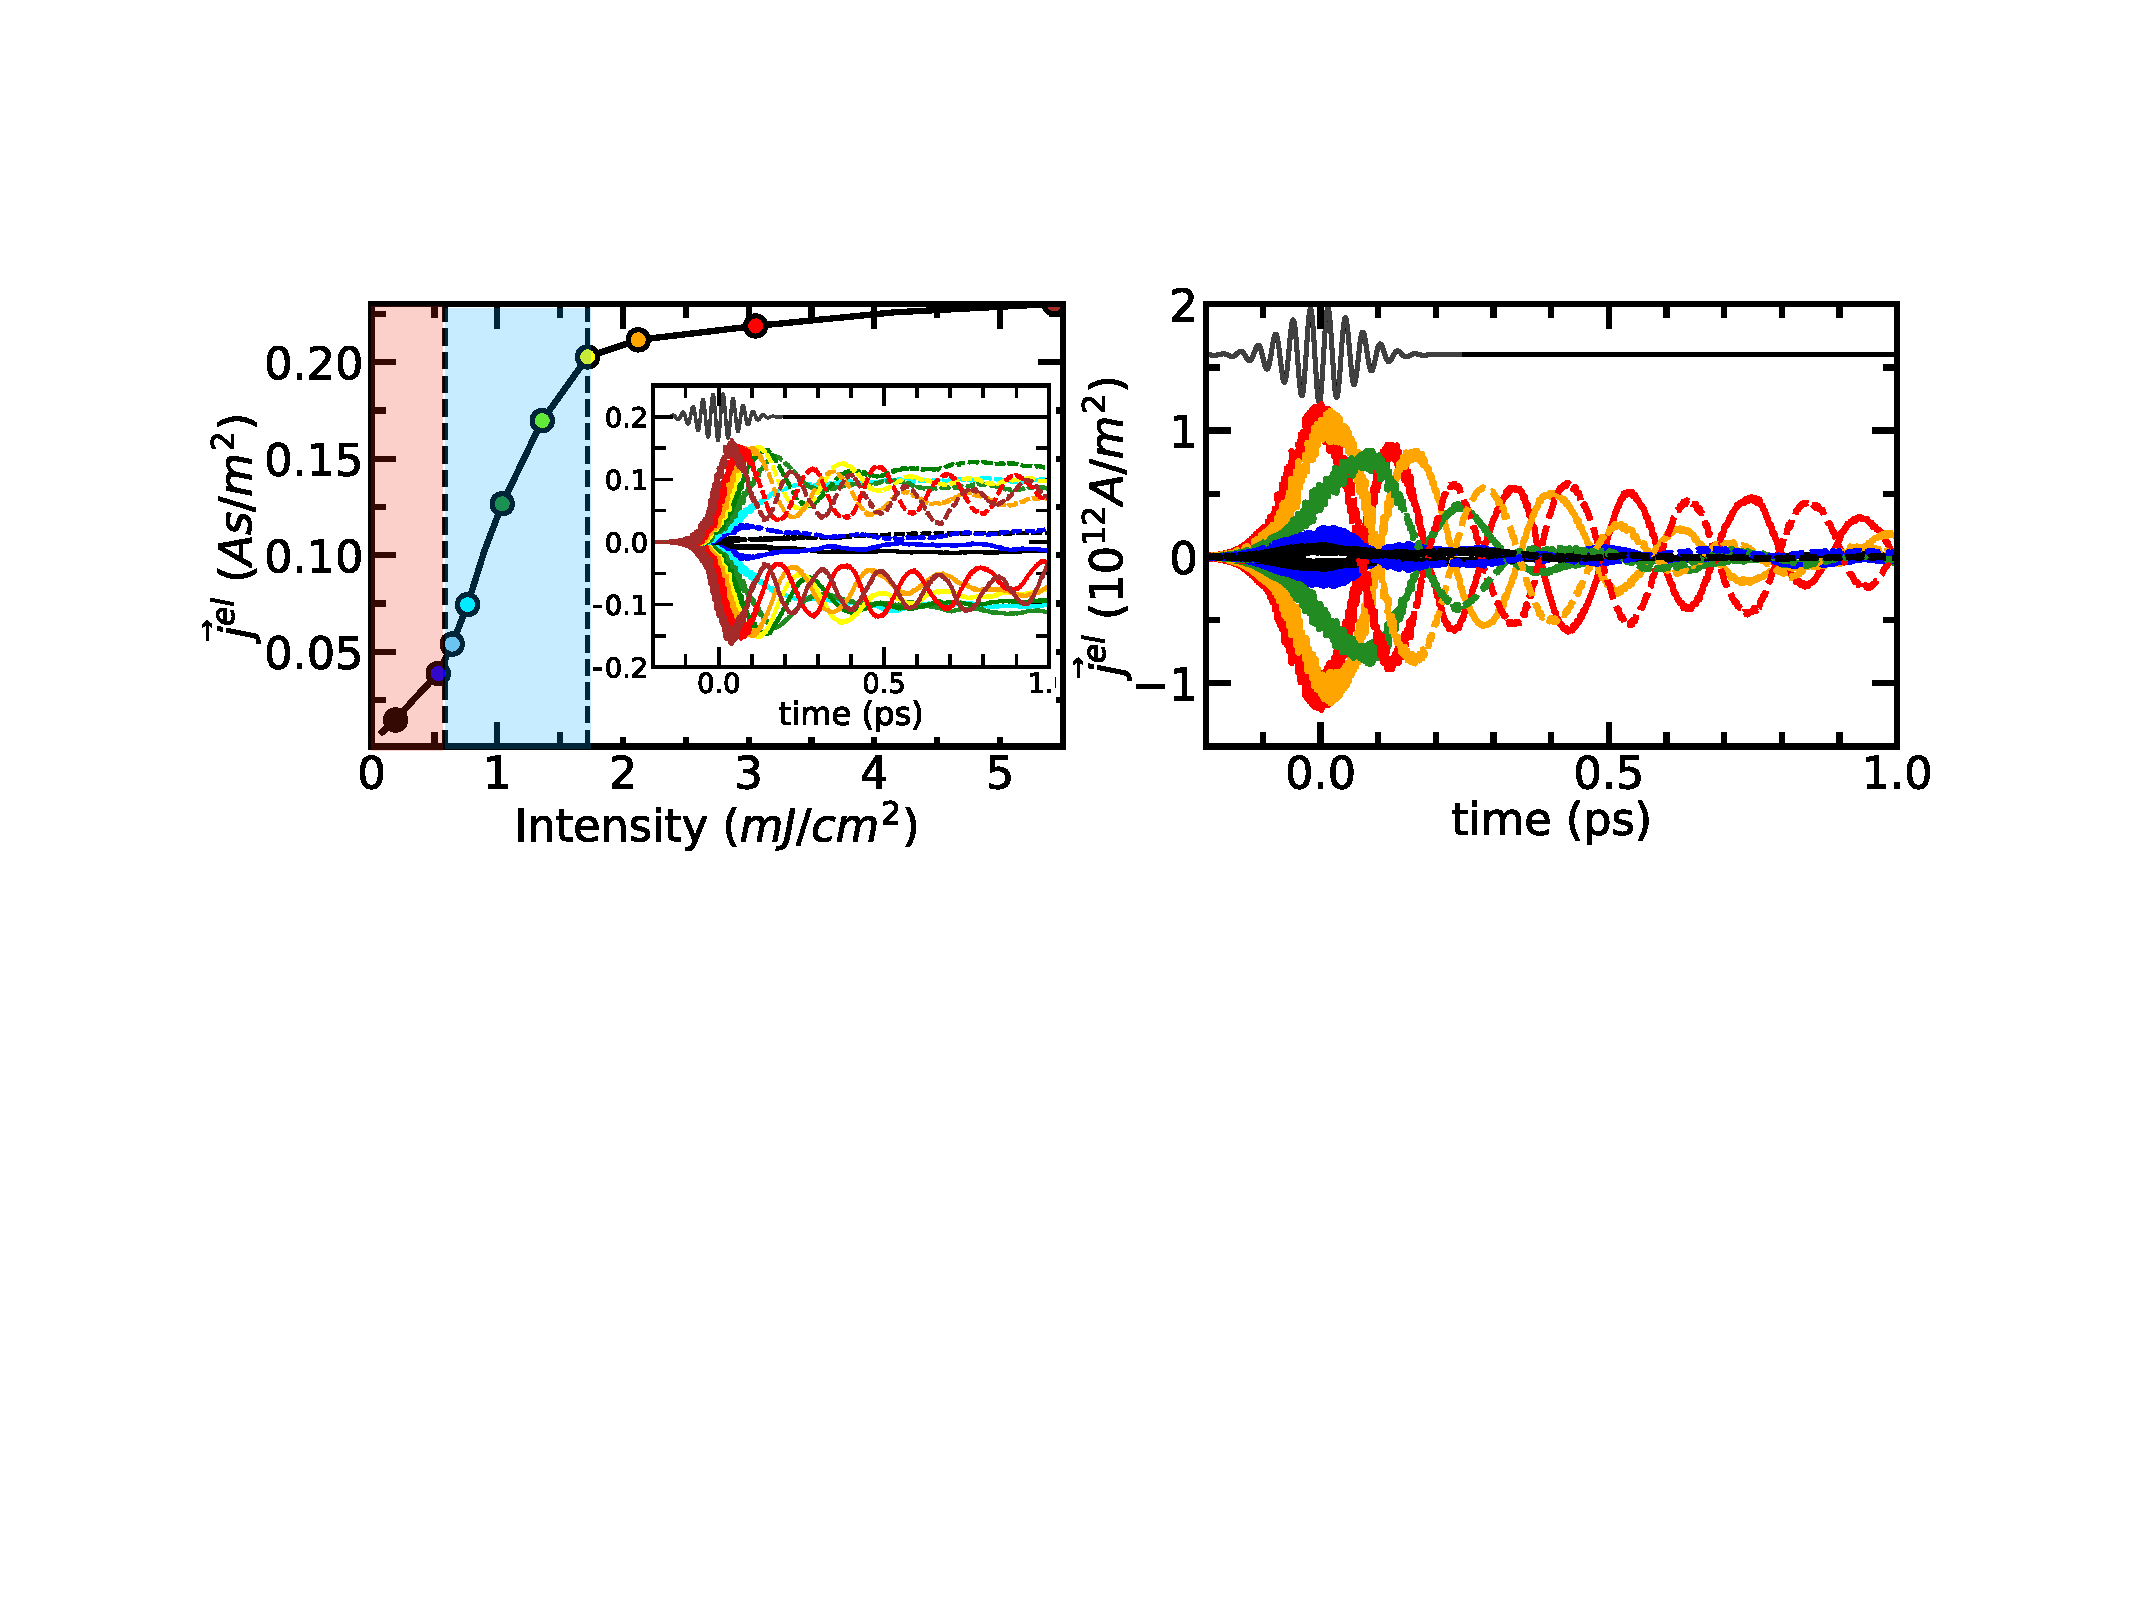
\includegraphics[width=1.0\linewidth]{figures/photocurrent_old}
    \caption{
        Simulated photocurrent of \(\mathrm{Pr_xCa_{1-x}MnO_3}\), as a function of light intensity and time after excitation. 
        Rapid enhancement of photocurrent (left) in indicative of a nonperturbative process beyond the frameworks of previously studied shift and ballistic current theories.
    }
    \label{fig:PCMO}
\end{figure}

To study this effect, we use a methodology based on real-time simulations of a first-principles based Hubbard model which treats all the relevant degrees of freedom, namely charge, spin, orbital and lattice, explicitly. 
Our methodology allows us to study transient effects such as THz oscillations and their decay on picosecond timescales, as well as current saturation at higher light intensities, all of which are inaccessible using perturbative frequency domain techniques that have been in use for BPVE. 

In this work, {\bf Tan} has supervised photocurrent simulations, {\bf Pemmaraju} has provided input on the handling of dissipative processes, and {\bf Ogitsu} has guided the research focus to questions that can be answered in greater detail using the \textsc{inq} code in the remaining project period. 
Follow-up work will utilize the exact-exchange functional features of the \textsc{inq} code to explore the impact of nonlocal exchange on photocurrents in these strongly correlated systems. GPU optimization of the \textsc{inq} code will be used to extend these simulations to the relevant time scales identified above.  

\subsubsection{Halide perovskite work}

High defect tolerance has been considered as a main reason for the long charge carrier lifetime and
high photoluminescence quantum yield in bulk lead halide perovskites (LHPs). On the other hand,
surface defects play a critical role in determining charge carrier dynamics and optical properties,
especially for LHP nanocrystals and quantum dots. Revealing the nature of surface defects and
developing strategy for their effective passivation are thus of strong interest.  {\bf Tan} and {\bf Ogitsu}, together with collaborators at UCSC~\cite{Smart2021}, have used first-principles calculations to reveal that interstitial and antisite defects in a prototypical LHP, CsPbBr$_3$, can have lower formation energy when they form at the surface instead of bulk while simultaneously creating deep trap states within the bandgap.  We show how to choose molecular ligands to passivating these defects, eliminating trap states in favor of shallow states, which enhances photoluminescence. (See Fig~\ref{fig:defect}) This work has implications for  the field of LHPs, especially LHP devices where interfacial chemistry plays an important role in the optoelectronic properties and stability.

This work forms the basis for planned real-time simulations of lossy processes at these defects in the LHPs, such as non-radiative recombination processes and dephasing, which are of fundamental interest for in optoelectronic applications. Even though typical RT-TDDFT simulations are shorter than the natural time scales of these processes, it has been demonstrated that their rates can still be extracted, by using a cumulant expansion approach~\cite{Qiao2020}. Scalability of the \textsc{inq} code will enable these calculations in challenging systems such as LHP surfaces defects, which contain a large number of electrons.     


\begin{figure}[h]
    \centering
    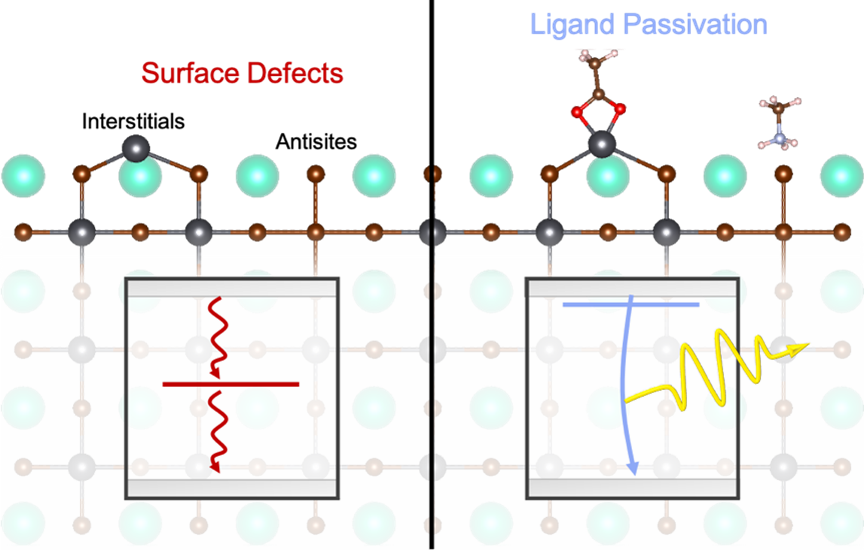
\includegraphics{figures/defect_passivation.png}
    \caption{
        Schematic atomic structure of defects at the surface of CsPbBr$_3$, which are susceptible to non-radiative recombination when unpassivated (left), but become less detrimental to radiative recombination when passivated (right).
    }
    \label{fig:defect}
\end{figure}

\textcolor{red}{Descriptions of selected type-B projects.}
\subsubsection{Ultrafast dynamics in strong-field ionized liquid water} 
\begin{figure}[h]
    \centering
    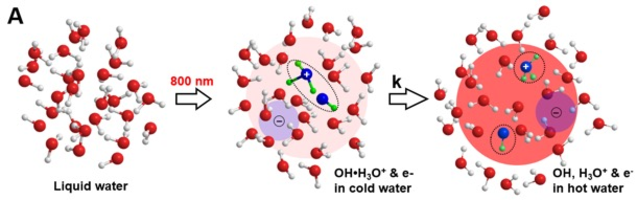
\includegraphics{figures/Water}
    \caption{
        The ionization of liquid water and formation of solvated \(\mathrm{H_3O^+}\), \(\mathrm{OH\cdot}\) radical and electron species is followed by the local thermalization involving energy exchange between the electronic and ionic degrees of freedom.
    }
    \label{fig:water}
\end{figure}

Photo-excitation induced structural dynamics in liquid water represents a paradigmatic case of excited state electron-ion dynamics in the condensed phase. 
In particular, the radiolysis of liquid water and its aftermath is a process of fundamental importance in a variety of technological contexts~\cite{Garrett2005} such energy harvesting, biochemistry, biomedicine, corrosion mitigation, etc. 
Therefore, investigating the interplay between the electronic and ionic degrees of freedom in photo-ionized liquid water on the femto-picosecond timescales relevant to the creation and transformation of short-lived reaction intermediates~\cite{Loh2020} is of interest to both experiment and theory.
Within the current funding period, NPNEQ researchers at SLAC collaborated with experimental teams working at SLAC's MeV-UED instrument to uncover the structural finger-prints of hydronium cation-hydroxyl radical pairs on femtosecond timescales in strong-field ionized liquid water (See Fig~\ref{fig:water}). 
In this study we deployed velocity-gauge real-time TDDFT as implemented within the \textsc{SALMON} code~\cite{salmon} to estimate the photo-ionization fraction in liquid water for experimentally relevant laser pulse parameters. 
Our simulations revealed a nonlinear multi-step photo-ionization process in liquid water subjected to high-intensity near-infrared radiation and our predicted excited electron energy distribution subsequently informed classical models of thermalization based on molecular dynamics. A manuscript summarizing the findings of our experiment-theory collaboration is currently under review at the journal \textit{Science}.
In the near future we plan to further extend our studies in this prototypical water system by simulating nonadiabatic Ehrenfest electron-ion dynamics during and after laser illumination using our RT-TDDFT platform \textsc{inq} and compare our results with recent ultrafast experiments. 
\subsubsection{WTe2 collaborations}

\subsubsection{Charge density wave melting in 2D materials}
In this experimental collaboration~\cite{Siddiqui2020}, we perform the first ultrafast investigation of TaTe$_2$, which exhibits unique charge density wave (CDW) and lattice structural order characterised by a transition upon cooling from stripe-like trimer chains into a (3x3) superstructure of trimer clusters. 

We develop computational models of the ultrafast photoinduced dynamics in TaTe$_2$, incorporating  electronic and atomic structure and their strong interactions to calculate the atomic trajectories. Density-functional calculations indicate that the initial quench is triggered by Ta trimer bonding to nonbonding transitions that destabilises the clusters, unlike CDW melting in other TaX$_2$ compounds. These predictions were verified by experimental work utilising MeV-scale ultrafast electron diffraction to resolve structural dynamics following intense pulsed laser excitation. We observe a rapid 1.4 ps melting of the low-temperature ordered state, followed by recovery of the clusters via thermalisation into a hot superstructure persisting for extended times.  Our work paves the way for further exploration and ultimately directed manipulation of the trimer superstructure for novel applications.



\section{Future Work}
\subsection{Code developments}
\subsubsection{Functionality additions to INQ}
\paragraph{Exact exchange and Axc}

Nonlocal functionals for Generalized Kohn-Sham (GKS) RT-TDDFT (Task 1.1)
% The need for more accurate descriptions of the electron density and its polarization response to perturbations across length scales is critical for real-time explorations of ultrafast dynamics. Field-driven excitations relevant to optical transitions require accurate band gaps and excited state evolution113, 116, 118. The potential to form self-trapped excited states, through electron-nuclear interactions, such as exciton-polaritons, places stringent accuracy requirements on exactly those areas where traditional (semi-)local exchange-correlation functionals fail due to significant self-interaction errors that limit or prevent electronic localization and the associated symmetry-breaking forces on local regions of the ionic lattice/nuclear coordinates112, 116, 144. 
% Nonlocal functionals featuring a fraction of Fock exchange provide one solution to this problem, generally reducing self-interaction, increasing bandwidth in the electronic DOS and reducing polarizabilities to values closer to experimental estimates118, 119. However, evaluation of the Fock operator within the exact-exchange formalism presents significant computational overhead for static calculations and can render time-dependent studies intractable. Such calculations, within a plane-wave basis (as proposed in this effort) present costs that scale as Ng log(Ng) Ne2, where Ng, the number of plane-wave basis functions can easily approach millions for large system sizes, even if the number of electrons, Ne, is only in the thousands. In partnership with NERSC, PI Prendergast recently succeeded in providing order of magnitude speed-up within the hybrid exact-exchange implementation for the open-source code, PWscf (part of the QuantumESPRESSO suite145) through (1) reorganization of the data layout when switching between the external local DFT self-consistent field loop and an internal non-local Fock matrix evaluation loop and (2) parallelization of the Fock matrix evaluation via band pairing146. These changes have been implemented within PWscf since version 6.1 of QuantumESPRESSO and recent applications include studies of transition metal oxides: variations in electronic DOS upon lithiation147 and significant improvements in transition state energetics for lithium ion transport148. 
% Furthermore, for large scale plane-wave applications, we will require convergent approximations to the Fock operator with further reductions in computational overhead, such as the Adaptively Compressed Exchange (ACE) approach of Lin149. In this development, the full exchange operator is replaced with a lower rank (Ne vs. Ng) approximant with convergence constraints. This has also been implemented with QuantumESPRESSO (since version 6.1) and another plane-wave implementation in the Discontinuous Galerkin DFT code (DGDFT150) and has been applied in benchmark studies of bulk silicon supercells and to the study of water adsorption on silicene151. ACE contrasts with previous efforts to exploit the locality of exchange interactions through transformations of the occupied Kohn-Sham orbital subspace to a basis of localized functions, such as maximally-localized Wannier functions (as developed by Car et al. 152 in the CP code within QuantumESPRESSO) or via recursive subspace bisection (as developed by Gygi et al. 153 in the Qbox code).
% The ACE approach for hybrid exact-exchange, combined with the parallel-transport (PT) gauge discussed previously represents a promising avenue (PT-ACE) towards efficient plane-wave basis set RT-TDDFT simulations133 within the Generalized Kohn-Sham (GKS) scheme. It is noted however by Jia et al133, that 1024 silicon atoms, running for ~30 fs employing PT-ACE still requires 1 week to compute on 2048 cores of Edison (at NERSC), although without PT-ACE, it might take a year to do the same. Therefore, there is clearly work still to be done to both improve the strong scaling of plane-wave implementations of hybrid exact-exchange within RT-TDDFT, by adapting promising algorithms like PT-ACE for scalable GPU-based architectures such as within Qbox. To this end, the simplifications and algorithmic improvements outlined above highlight potential opportunities to offload significant computational work while leveraging hardware specific implementations of standard matrix-multiply and fast Fourier transform routines. 
% (Task 1.1) In view of the above, the NPNEQ team will develop GKS RT-TDDFT functionality featuring range-separated hybrid XC functionals by leveraging  algorithms such as PT-ACE within the scalable Qbox framework.  


\paragraph{Non-collinear magnetism and spin-orbit}
Spin-orbit coupling for dynamics (Task 1.3)
 
% In time-independent problems the description of spin-orbit coupling is necessary to reproduce accurate atomic energies and level splitting. In thermal equilibrium the spin state and the existence of magnetism is determined by free energy minimization. In time-dependent problems the situation is more complicated, since the only way to change the spin state is by an external magnetic field or internally by spin-orbit coupling. Processes like ultrafast demagnetization can be phenomenologically explained by models that assume kinetics upon free energy models 162 but a practical microscopic model is still absent.
% Specifically, we will implement spin-orbit coupling (SOC) dynamics, which will significantly improve fidelity of quantum dynamics simulations of functional materials that often comprise transition metals and exhibit complex magnetism. Our implementation of SOC for the planewave basis will not use the projection approximation that virtually all the currently existing (TD)DFT software relies on; as it has been shown to be inappropriate for a description of time dependent quantum mechanical evolution 163.
% The ubiquitous projection approximation allows to use a natural representation of the spin-orbit interaction by an additive term of the type  with prefactors calculated at the atomic (pseudopotential) level (   is a local projection of the electronic orbital angular momentum). The definition of  depends on ionic positions, which are varying dynamically along with the simulation. Effectively this defines a representation in a curved and changing Hilbert space that is very complex to code163 .
% Although this picture of SO coupling it is usually justified by the dominance of localized orbitals, in the non-adiabatic context, the simplifications of the projection method carry a heavy complexity cost. Additionally, a time-dependent theory of magnetism is necessarily non-colinear, in order to continuously connect different spin configurations.
% Time-dependency, non-colinear magnetism and dynamical ions (coupled to both electron-orbital and spin) call for a new approach to the problem of spin in first-principles simulations. Our alternative strategy starts from the the Breit-Pauli Hamiltonian in the two component spinor algebra 164. The Breit-Pauli terms incorporate scalar relativistic corrections to the non-relativistic Hamiltonian, and contain spin-explicit terms describing the interaction between the orbital magnetic moments and spin magnetic moments:

% where  is the gradient (force) of the nuclear potential. This part of the Hamiltonian contains two-body terms that are unacceptable in the Kohn-Sham theory, therefore we will use the gradient of self-consistent effective potential as presented by Krieger et al.
% This representation of the SO is independent on the labeling of ions and not-explicitly dependent on the ion positions (only through the potential); it doesn’t rely on a local projection of the angular momentum and it is more suitable for a time dependent treatment with co-evolving ions. In the same way that a quantum ion-electron interaction leads to advanced picture of electron-phonon coupling (a two-temperature system),128 this development will lead to a fuller picture to guide advances of effective models of spin-lattice-electron dynamics166. This is important, in particular, to handle time evolution of Weyl points driven by lattice motion or circularly polarized light, addressing the needs for modeling experimental efforts described in other sections. 

\paragraph{Spiral boundary conditions}

\paragraph{Beyond Ehrenfest dynamics} 
Mention: Electron-phonon development from stopping power.  Figure.

\paragraph{Interfacing \textsc{inq} with Tight-Binding codes}

We plan to use \textsc{inq} in combination with our tight-binding dynamics code (Section.~\ref{sec:tight-binding}) for parameter extraction and for identification of the relevant degrees of freedom to be retained in these downfolded models. Having a well-defined interface for these tasks will accelerate projects of the sort described in Sections~\ref{sec:BPVE},~\ref{sec:tight-binding}. Dynamical Wannierization along TDDFT trajectories will provide Hamiltonian matrix elements for the construction of these models, generalizing an approach previously taken for Wannierization along classical MD trajectories~\cite{Abramovitch2021}. These script-heavy workflows will be greatly simplified in \textsc{inq}, which will include a language-level interface to the \textsc{Wannier90} library~\cite{Mostofi2008}. Other types of script-heavy workflows, especially those with high throughput aspects, will benefit similarly from the modularity of \textsc{inq}, which makes scripting and post-processing obsolete in favor of programmability within the single-language \textsc{inq} framework.

Scientifically, having the \textsc{inq} code coupled to local-basis models will enable the exploration of research questions relating to the dynamics of localization. The appropriate parameterization of tight-binding models suitable for describing non-adiabatic dynamics remains an open question, and similar questions remain in the propagation of local orbitals, particularly close to metallicity~\cite{Yost2019}. With these tools, we will study how orbital localization arises from decoherence, finite-temperature effects, and scattering processes.  

\subsection{Science Applications}
\subsubsection{Spin dynamics in layered anti-ferromagnets}
Several ongoing projects involving close collaboration between experimental efforts and theory from this team are in progress.

In collaboration with {\bf Tan} and {\bf Pemmaraju}, {\bf Lindenberg} has been investigating the ultrafast dynamical response of two-dimensional antiferromagnetic materials.
In antiferromagnets, electron exchange interactions result in antiparallel or non-collinear microscopic spin correlations with negligible macroscopic magnetization.
Given their low-loss, intrinsic THz frequencies, and insensitivity to stray fields, antiferromagnetic spintronics holds great potential in realizing high-speed communications and new types of information storage technologies. 
Atomically-thin van der Waals crystals like \(\mathrm{FePS_3}\), \(\mathrm{NiPS_3}\) and \(\mathrm{MnPS_3}\) represent a new type of antiferromagnetic materials class with strong 2D quantum confinement and the ability to tune this functionality at high speed and with low energy cost taking advantage of the weak interlayer van der Waals bond.
In initial work we have carried out time domain THz emission spectroscopy probing the ultrafast dynamics of the magnetization in exfoliated flakes of \(\mathrm{NiPS_3}\).
In these experiments an ultrafast optical pump pulse excites above band gap at \(400~\mathrm{nm}\) to create free carriers which then couple to the intrinsic magnetization of the material.
By detecting the emitted THz fields from the sample we probe the time-dependent free (associated with the flow of electrons) and bound (associated with the time-dependent magnetization) currents.  Following directly from Maxwell’s equations one finds: 

\begin{equation}
\mathbf{E}_\text{THz} \propto \frac{\partial\mathbf{J}}{\partial t}+ \frac{\partial}{\partial t} (\nabla \times \mathbf{M})
\end{equation}

where \(\mathbf{J}\) is the free current and \(\mathbf{M}\) is magnetization. 
Fig.~1 shows the experimentally measured THz waveform and the peak-to-peak emission amplitude as a function of temperature, showing an enhancement at the Neel temperature.
This demonstrates the sensitivity of the measurement to the intrinsic antiferromagnetic dynamics.
Further, by measuring the polarization state of the emitted THz fields one can extract information about the crystallographic directions of the associated currents.
We find there are two contributions to the measured fields, involving a current normal to the sample surface associated with the separation of electrons and holes at the surface superposed on a bound current likely associated with an induced rotation of the initially in-plane antiferromagnetic magnetization state.
Further spectral analysis of the emitted fields may allow us to extract information about particular magnons associated with the light-induced response.
This work opens up new possibilities for controlling the properties of antiferromagnetic materials on ultrafast time-scales. 
Ongoing work additionally involves upcoming experiments at the SLAC National Accelerator Laboratory Ultrafast Electron Diffraction facility where we will in parallel investigate the correlated structural dynamics under similar photoexcitation conditions.

\begin{figure}[ht]
    \centering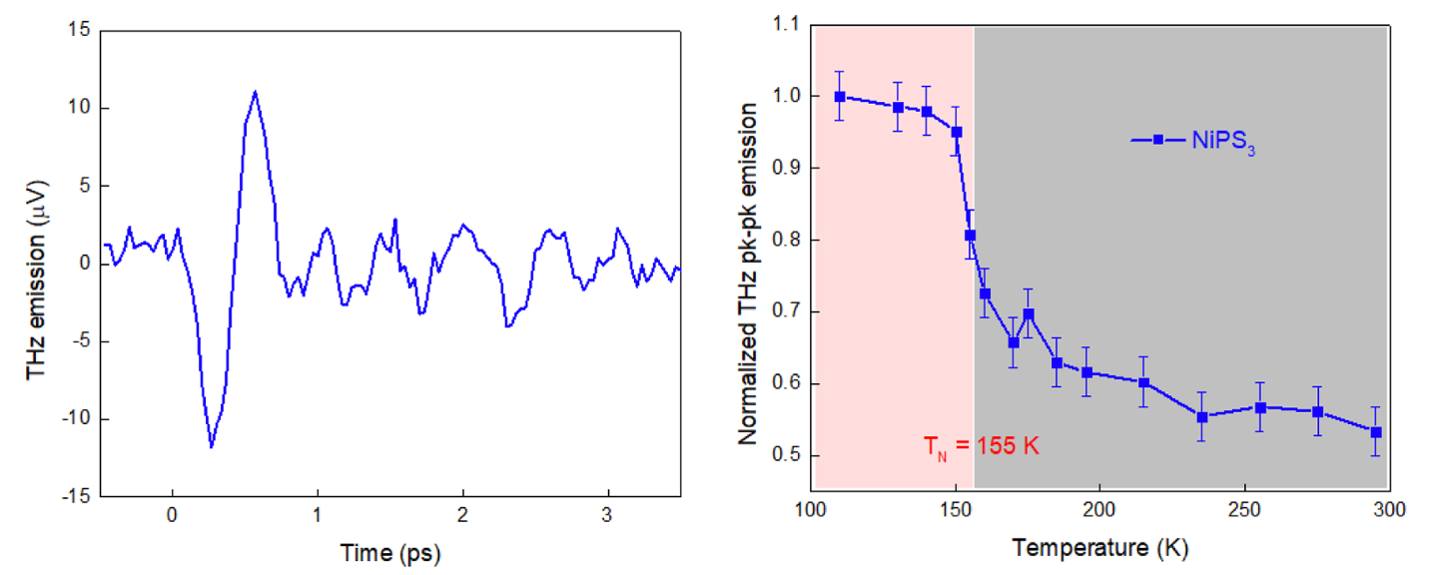
\includegraphics[width=1.0\linewidth]{figures/NiPS3}
    \caption{
        (left)  Measured THz electric field waveform emitted from NiPS3 antiferromagnetic sample under femtosecond \(400~\mathrm{nm}\) excitation.
        (right) Peak THz emission amplitude as a function of temperature, showing strong enhancement at the Neel temperature (\(155~\mathrm{K}\)), showing direct sensitivity to time-dependent magnetization.
    }
    \label{fig:NiPS3}
\end{figure}

In conjunction with this experimental work, {\bf Tan} and {\bf Pemmaraju} are investigating a number of theoretical approaches to this problem.
First, static, first-principles density functional theory are used to solve for the electronic structure, phononic properties, and electron-phonon interactions of the \(\mathrm{NiPS_3}\) materials system. 
Second, the RT-TDDFT approach will be used to directly simulate density and spin fluctuations in time using the INQ code.
The evolution of the calculated diffraction intensities of the spin, charge and orbital patterns will provide dynamics of the order parameters to assist the experimental time-resolved diffraction study.
Trajectories will be examined to understand the structural and electronic mechanisms behind the evolution of spin order peaks, and their associated time scales. 
Finally, the RT-TDDFT simulations will provide data for parameterization of a model for long-wavelength magnon simulations. 
This semi-classical approach involves the construction of an effective spin Hamiltonian consisting of Zeeman, exchange and anisotropic magnetic interactions, with parameters extracted from the INQ code. 
This Hamiltonian will be solved for large magnetic supercell to produce the spin-wave dispersions. 
Development of this model will be accelerated by the team’s recent experience with similar models for 2D TMDCs and manganites~\cite{Siddiqui2020, Rajpurohit2020}. 
As a by-product of this work, the \textsc{inq} code will contain an interface that will facilitate user extraction of parameters for model simulations.

\subsubsection{Halide Perovskites/Photovoltaics/Exciton dynamics}

\subsubsection{Nonlinear nonequilbrium response in topological materials}

Nonlinear optical phenomena arise when light at sufficiently high intensities interacts with matter. Nonlinear response underlies technologically important physical effects including shift-currents, harmonic generation and frequency upconversion in photovoltaic and optoelectronics applications among others.  Recent insights that nonlinear responses are intimately tied to the fundamental topological properties of the quantum materials, has added to the interest in controlling the excited states of these systems with  ultrafast pump-probe and nonlinear multidimensional spectroscopies.

The computational studies proposed in this project are inspired by recent joint experiment-theory results reported by PIs Lindenberg and Pemmaraju on ultrafast nonlinear responses in the Weyl semimetal WTe$_2$ . Our studies showed that terahertz frequency light pulses induce large amplitude interlayer shear strains in WTe$_2$ , modulating its symmetry and potentially its topological phase. The THz induced shear strains in WTe$_2$ were also found to be associated with a large transient modulation of the second harmonic generation (SHG) response whereby in the THz driven sample, the SHG response is dramatically reduced compared to noncentrosymmetic bulk WTe However since the low order nonlinear response in materials is fundamentally connected with topological quantities such as the Berry connection and Berry curvature , the question remains as to whether the observed transient reduction in SHG is a signature of a topological phase transition involving the annihilation of Weyl nodes in the Bloch band structure or that of a structural transition to a centrosymmetric geometry.

We will investigate the electronic vs structural origins of recently observed large transient changes in the second harmonic response of the Weyl semimetal WTe$_2$ in response to terahertz driven lattice modulations. The relationship between symmetry, topology and SHG response in WTe$_2$ will be investigated using both frequency and time-domain approaches. Simulations of SHG response in \textsc{inq} will go beyond the Born-Oppenheimer approximation to model intrinsic non-equilibrium states involving transient field-driven modulations of the electrons and holes near the Weyl band crossing points. Utilizing the Ehrenfest dynamics capability of the \textsc{inq} code, we plan to investigate the role of transient in-plane currents in driving the observed 0.24 THz shear-shear responses in WTe$_2$, and the role of electron doping in tuning these responses. Such studies will contribute significantly to a detailed material specific understanding of ultrafast nonlinear response in topological materials within the TMDC family and beyond.

\clearpage

\section{Management Plan}
\label{sec:manage}

During the first two years of our project, our essential management strategy was based on the geographical proximity of the team and its fairly small size. We had relatively frequent meetings, through which detail of our approaches were determined based on extensive discussions and consensus building with the shared goal of advancement of ultrafast science through development and distribution of GPU enabled RT-TDDFT software and collaborative research using the software. 

The software development and validation teams held two two-hour meetings per week where {\bf Tadashi Ogitsu (director)} initiated discussions, and the task leads, {\bf Alfredo Correa (software design)}, {\bf Xavier Andrade (GPU adoption)} and {\bf Das Pemmeraju (validation)} formulated a short to mid term strategy towards the initial goal of completing GPU enabled MPI parallel RT-TDDFT software named \textsc{inq}, discussed the progress status, revised strategy if deemed necessary.

Important factors considered in developing the strategy were the status of ever-evolving HPC systems and needs of the scientific community, while being clearly aware of resource restrictions on our development scope. 
This practice is crucial for the success of our project due to their tight inter-dependencies, rapid and dramatic change in the hardware architecture of HPC systems, such as dual memory spaces and redundant interconnects introduced by the addition of GPU to CPU, as well as relatively immature current status of RT-TDDFT, where significant number of new methodological and algorithmic developments are being expected. 

Accordingly, we focused on developing and maintaining GPU-ready libraries for commonly used DFT and TDDFT routines so as to provide maximum flexibility in transferability of the software for future DOE leadership class HPC systems, which may have diverse architectural design, while providing a developer friendly software platform to the (TD)DFT community, maximizing external collaborators participation to the software development. 
This approach is unique in that currently popular ab-initio software, such as VASP, Quantum-Espresso, NWChem, focus on providing rather a complete package being developed by small to modest number of major contributors presumably owing to longer history of DFT software development compared to that of TDDFT.

Two staff scientists, {\bf Correa} and {\bf Andrade}, at 0.5~FTE level were therefore dedicated to the design and implementation of \textsc{inq}. 
{\bf Correa} has an extensive experience in implementing TDDFT algorithm into Qbox code written by Francois Gygi in C++ computer language and MPI parallelization. 
In addition, he has been developing a C++ template library named \textsc{multi} for the QMCPACK project.
Design of \textsc{multi} shares the same philosophy with our project: provide basic libraries that are designed to be used by scientists (not expert programmers), while securing good performance on complex HPC systems such as a CPU+GPU hybrid computer. 
{\bf Andrade} has an extensive experience in developing another TDDFT open software named \textsc{octopus}, in particular, he contributed to its GPU optimization.  

Based on their experiences, {\bf Correa} assumed responsibilities on overall design of the \textsc{inq} library and software development progress, while {\bf Andrade} assumed responsibility on the design and implementation intimately related to GPU optimization. 
They held nearly daily communication in the earlier stage to develop software design guidelines in order to maximize balance between software programmability, transferability and performance. 

Systematic testing is crucial for scientific software development, 
ensuring reliable and reproducible results are produced. 
{\bf Pemmaraju} (0.1~FTE) together with his PD, Alexey Kertzev (1~PD), who are experts on TDDFT simulations have developed software testing protocols, which means identifying the type of systems, simulations and physical quantities to be compared against well established codes such as QE, 
\textsc{octopus} and QB@ll. 
Testing suites are distributed together with the software in order for the external collaborators to ensure correctness in their platforms.
{\bf Pemmeraju} assumed responsibility in designing and performing \textsc{inq} integration tests.

While our \textsc{inq} software was being developed, the experiments ({\bf Aaron Lindenberg (experimental validation)}) and interpretation ({\bf Liang Tan (interpretation)}) team was tasked to perform more elaborate scientific research that would use \textsc{inq} code when it become available. 
They assumed responsibilities on designing and conducting theory and experiments collaboratively, which would take full advantage of \textsc{inq} code when it become available. Even though experimental work during the pandemic has been limited, we have collected more experimental data recently, which contain new observations that are forming the basis of planned simulations (Sec.~\ref{sec:2dafm}). 
{\bf Lindenberg}'s PD, {\bf Xiao (0.5~PD)}, very recently started an assistant Professor position at University of Wisconsin, Madison and are planning to continue the collaboration with us on the subject of ultrafast science.

As the experimental validation team was impacted by the pandemic, {\bf Tan} assumed other crucial responsibilities: the development of software for tight-binding coupled spin-electron-ion dynamics to augment our software validation effort at long time- and length-scales. 
These developments have led to new scientific questions to be studied with \textsc{inq} (Sec.~\ref{sec:BPVE}), and to external collaborations that would contribute to the software validation and expand the \textsc{inq} user base (Sec.~\ref{sec:collaborative}). 
The original tight-binding software was developed by  Rajpurohit (1~PD) with Prof. Peter Bl\"{o}chl. 
She is currently developing a new version for 2D layered systems under {\bf Tan}'s supervision, which will be used for more elaborate software validation effort with {\bf Lindenberg} team during the second half of our project.
The tight-binding code will fully leverage information generated by \textsc{inq}, such as electron-ion coupling parameters in non-perturbative limit (Sec.\ref{sec:future-tb}). 
{\bf Tan} and {\bf Prendergast} (internal advisor) publicized our project via conference/workshop organization and presentations. 

In order to facilitate internal and external collaborations, we held all-hands meetings approximately every 6 weeks, for research planning and reporting.
These meetings were held in-person at LLNL/LBNL/SLAC until early 2020, then switched to online meetings.
For the technical discussions for the internal collaboration, we started separate monthly meeting in early 2021, when experimental research became gradually feasible. 
Regular participants were {\bf Linenberg}, {\bf Xiao}, {\bf Pemmaraju}, {\bf Tan}, {\bf Rajpurohit} and {\bf Ogitsu} and the rest of members as necessary.

We invited numerous researchers from HPC and ultrafast science communities to these meetings. 
David Richards (lead of LLNL HPC procurement team) gave us great insights on the current and future HPC situation from hardware and system software perspectives, 
Prof. Yuan Ping (UCSC) and student presented her density matrix based spin dynamics code, which lead to our mutual collaboration on charge carrier decay at defects in perovskite quantum dots and a publication~\cite{Smart2021}. 
Prof. David Strubbe (U.C. Merced) gave a seminar on the application of RT-TDDFT to ultra-strong shock physics, which led to invitation to the 2020 Electronic Structure workshop, where {\bf Ogitsu} introduced NPNEQ project to the participants followed by \textsc{inq} tutorial by {\bf Andrade} and {\bf Correa}. 
A meeting with Francois Gygi was held to exchange information about our respective software development plans (\textsc{inq} and \textsc{Qbox}). 
We visited Prof. Lin Lin (UC Berkeley) to learn about the state-of-art time integration scheme and GPU adoption. 
Prof. Carsten Ullrich (U. Missouri) presented methodological developments including a new exchange-correlation kernel for RT-TDDFT. 
Prof. John Rehr gave a presentation about FEFF project.

We have been inviting SAB members one by one to resolve international scheduling constraints. 
Prof. Yabana (U. Tsukuba)  gave a lecture on his \textsc{salmon} project and discussed various aspects of software development and distribution. 
Prof. Emilio Artacho (Cambridge) is scheduled to participate in a discussion about software development and distribution plans of NPNEQ and his project (CECAM's Electronic Structure Library) after the midterm review.

The director, {\bf Ogitsu} (0.25FTE), oversaw all activities and communicated with the members assisting redirecting effort, for instance, of the activities impacted by the pandemic.



\clearpage


\section{Development And Utilization Of Unique Facilities, Capabilities, Or Approaches}
\label{sec:development}
{\small\color{red}
\begin{itemize}
\item 3 pages max
    \item Describe the most important instrumentation, computer codes, and databases purchased or developed for the project and their pertinent capabilities. Provide 
    \begin{enumerate}
        \item software release numbers,
        \item user metric where available,
        
        \item citations of the accompanying publication of new software releases.
        \item Links to software and database download sites should be provided in separate spreadsheet (see below).
        \item Also describe any unique shared facilities (including national user facilities) that have been or will be used for the project, including ALCC or INCITE awards.
    \end{enumerate}    
\end{itemize}

}

Grand Challenge 

Outreach summer school director, two students.

QMCPACK library

As requested by the program, one of the central objectives of the first half of the NPNEQ center was the delivery of a performant GPU DFT code to tackle non-perturbative and non-equilibrium phenomena studied by the center.
INQ is a new implementation of density functional theory (DFT) and time-dependent DFT (TDDFT) written from scratch to work on graphical processing units (GPUs).  
Besides GPU support,INQ makes use of modern code design features and takes advantage of newly available hardware.
By designing the code around algorithms, rather than against specific implementations and numerical  libraries, we aim to provide a concise and modular code.
The result is a fairly complete DFT/TDDFT implementation in roughly 12,000 lines of open-source C++code representing a modular platform for community-driven application development on emerging high-performance computing architectures.

Talk about libraries used by QMCPACK also.


Outreach activities include the organization of a symposium at the 2021 Molecular Foundry Annual User meeting (August 19-20, 2021). The symposium, entitled “Non-Equilibrium and Non-Perturbative Experimental and Theoretical Methods for Dynamical Science”, aims to survey recent progress in manipulation, measurement, and simulation of non-equilibrium dynamics. Alongside the symposium organization, the INQ team will also be presenting a tutorial-style introduction to the INQ code during the Molecular Foundry User Meeting, as a way to introduce the code to the electronic structure community. 

\clearpage
\section{Publications, September 2019-Present}
\label{sec:publications}

\subsection{A-type}
Publications that were solely supported by this project and those in collaboration with others that are based on work which was intellectually driven by this project.
\begin{enumerate}
    \item \textcolor{blue}{Xavier Andrade}, \textcolor{blue}{Chaitanya Das Pemmaraju}, {\bf Alexy Kartsev}, \textcolor{blue}{Liang Z. Tan}, {\bf Sangeeta Rajpurohit}, {\bf Jun Xiao},  \textcolor{blue}{Aaron Lindenberg}, \textcolor{blue}{Tadashi Ogitsu}, and \textcolor{blue}{Alfredo Correa}, "INQ, a modern GPU-accelerated computational framework for (time-dependent) density functional theory", submitted on June 7, \url{https://arxiv.org/abs/2106.03872}.
    \item {\bf Sangeeta Rajpurohit}, \textcolor{blue}{C. Das Pemmeraju}, \textcolor{blue}{Tadashi Ogitsu}, and \textcolor{blue}{Liang Z. Tan}, "A non-perturbative study of bulk photovoltaic effect enhanced by an optically induced phase transition", submitted on May 24, 2021, \url{https://arxiv.org/abs/2105.11310}.
    \item Tyler J. Smart, Hiroyuki Takenaka, Tuan Anh Pham, \textcolor{blue}{Liang Z. Tan}, Jin Z. Zhang, \textcolor{blue}{Tadashi Ogitsu}, and Yuan Ping, "Enhancing Defect Tolerance with Ligands at the Surface of Lead Halide Perovskites", submitted on April 12, 2021.
\end{enumerate}

\subsection{B-type}

Collaborative publications jointly supported by this project and other programs or agencies.


\begin{enumerate}
    \item Jorge Kohanoff, \textcolor{blue}{Alfredo Correa}, Gleb Gribakin, Conrad Johnston, Andr\'{e}s Sa\'{u}l, "Radioactive decay of $^{60}$Sr in cement: a non-equilibrium first-principles investigation", submitted in May 2021.\\
    (Note: The Qball TDDFT code was used to calculate the electronic shake-off process of nuclear decay in a solid for the first time.)

    \item Khalid M. Siddiqui1, Daniel B. Durham, Frederick Cropp, Colin Ophus, {\bf Sangeeta Rajpurohit}, Yanglin Zhu, Johan D. Carlstr\"{o}m, Camille Stavrakas, Zhiqiang Mao, Archana Raja, Pietro Musumeci, \textcolor{blue}{Liang Z. Tan}, Andrew M. Minor, Daniele Filippetto, and Robert A. Kaindl, "Ultrafast optical melting of trimer superstructure in layered 1T’-TaTe2" submitted.  arXiv:2009.02891

    \item Edbert J. Sie, Clara M. Nyby, \textcolor{blue}{C. D. Pemmaraju}, Christina A. C. Garcia11, Yaxian Wang, Burak Guzelturk, Chenyi Xia, {\bf Jun Xiao}, Andrey Poletayev, B. K. Ofori-Okai, Matthias C. Hoffmann, Su Ji Park, Xiaozhe Shen, Jie Yang, Renkai Li, Alexander H. Reid, Stephen Weathersby, Philipp Muscher, Nathan Finney, Daniel Rhodes, Luis Balicas, James Hone, William Chueh, Thomas P. Devereaux, Prineha Narang,Tony F. Heinz, Xijie Wang, \textcolor{blue}{Aaron M. Lindenberg}, "Ultrathin Terahertz Waveplate Using an Anisotropic Semimetal" under review.
    
    \item Ming-Fu Lin, Narendra Singh, Shujia Liang, Mianzhen Mo, Pedro Nunes, Kathryn Ledbetter, Jie Yang, Michael Kozina, Stephen Weathersby, Xiaozhe Shen, Amy Cordones-Hahn, Thomas Wolf, Kelly Gaffney, \textcolor{blue}{C. D. Pemmaraju}, Matthias Ihme, Xijie Wang, "Imaging the solvated hydronium cation and hydroxyl radical in the ionized liquid water", under review.

    \item Khalid M. Siddiqui, Daniel B. Durham, Frederick Cropp, Colin Ophus, {\bf Sangeeta Rajpurohit}, Yanglin Zhu, Johan D. Carlström, Camille Stavrakas, Zhiqiang Mao, Archana Raja, Pietro Musumeci, \textcolor{blue}{Liang Z. Tan}, Andrew M. Minor, Daniele Filippetto, Robert A. Kaindl, "Ultrafast optical melting of trimer superstructure in layered 1T'-TaTe2", {\it Comm. Phys.} accepted June 8, 2021, https://arxiv.org/abs/2009.02891 

    \item  {\bf Sangeeta Rajpurohit}, \textcolor{blue}{Liang Z. Tan},  Christian Jooss, and P. E. Bl\"ochl, , "Ultrafast spin-nematic and ferroelectric phase transitions induced by femtosecond light pulses", {\it Phys. Rev. B} {\bf 102}, 174430-6 (2020). Published on Nov 18, 2020.

    \item Edwin E. Quashie, Rafi Ullah, \textcolor{blue}{Xavier Andrade}, and \textcolor{blue}{Alfredo A. Correa}, "Effect of chemical disorder on the electronic stopping of solid solution alloys", {\it Acta Mater.} {\bf 196}, 576-583 (2020). Published on Sep 1, 2020.\\
    (Note: The Qball TDDFT code was used to calculate full atomistic effects in the electronic-ion coupling and electronic response at extremely low ion velocities.)
        

    \item {\bf Jun Xiao}, Ying Wang, Hua Wang, \textcolor{blue}{C. D. Pemmaraju}, Siqi Wang, Philipp Muscher, Edbert J. Sie, Clara M. Nyby, Thomas P. Devereaux, Xiaofeng Qian, Xiang Zhang and \textcolor{blue}{Aaron M. Lindenberg}, "Berry curvature memory through electrically driven stacking transitions", {\it Nature Physics} {\bf 16}, 1028-1034 (2020). Submitted on Dec 1, 2019, published online on June 29, 2020.

    \item  Luke McClintock, Rui Xiao, Yasen Hou, Clinton Gibson, Henry Clark Travaglini, {\bf David Abramovitch}, \textcolor{blue}{Liang Z. Tan}, Ramazan Tugrul Senger, Yongping Fu, Song Jin, and Dong Yu, "Temperature and Gate Dependence of Carrier Diffusion in Single Crystal Methylammonium Lead Iodide Perovskite Microstructures", {\it J. Phys. Chem. Lett.} {\bf 11}, 1000-1006 (2020). Published on Jan 20, 2020.

\end{enumerate}

\clearpage

\appendix

\section{Biographical Sketches of Senior Investigators}
\label{sec:bio}
%\textcolor{red}{Provide a biographical sketch (CV) for each senior person (can be the same as for the management review or in original proposal), including those at partner institutions. Senior personnel are all those named on the staffing table, whether or not they receive funding from the CMS project. Provide concise vitae, listing professional and academic essentials and complete contact information. Include a list of up to ten publications that are most pertinent to the project.}
\subsection*{Tadashi Ogitsu, PI}

Lawrence Livermore National Laboratory: Senior Staff Scientist, Quantum Simulation Group, Materials Science Division, Physical and Life Sciences Directorate; 926-422-8511; ogitsu1@llnl.gov

\subsubsection*{Education and Training}

\begin{table}[ht]
\centering
\begin{tabular}{llll} 
University of Tsukuba  & Energy Conversion Engineering & B.A. & 1989 \\ 
University of Tsukuba & Materials Sciences & M.S. & 1991 \\
University of Tsukuba & Materials Sciences & Ph.D. & 1994 \\
\end{tabular}
\end{table}

\subsubsection*{Research and Professional Experience}

\begin{table}[ht]
\centering
\begin{tabular}{ll} 
Senior Staff Scientist in QSG, Lawrence Livermore National Laboratory & 2016-present\\
Staff Scientist in QSG, Lawrence Livermore National Laboratory & 2001-2016 \\
Postdoctoral Fellow, University of Illinois at Urbana-Champaign & 1998-2001 \\
Research Associate, Institute for Solid State Physics, University of Tokyo & 1994-1998 \\
\end{tabular}
\end{table}

\subsubsection*{Publications}
\begin{enumerate}
    \item T. Ogitsu, A. Fernandez-Pañella, S. Hamel, A.A. Correa, D. Prendergast, C.D. Pemmaraju, Y. Ping, “Ab initio modeling of nonequilibrium electron-ion dynamics of iron in the warm dense matter regime,” {\it Phys. Rev. B} {\bf 97}, 214203 (2018).
    \item B. Cho, T. Ogitsu, K. Engelhorn, A. Correa, Y. Ping, J. Lee, L. Bae, D. Prendergast, R. Falcone, P. Heimann, “Measurement of Electron-Ion Relaxation in Warm Dense Copper,” {\it Sci. Rep.} {\bf 6}, 18843 (2016).
    \item T. Ogitsu, Y. Ping, A. Correa, B.-i. Cho, P. Heimann, E. Schwegler, J. Cao, G.W. Collins, “Ballistic electron transport in non-equilibrium warm dense gold,” {\it High Energy Density Physics} {\bf 8}, 303 (2012).
    \item B.I. Cho, P.A. Heimann, K. Engelhorn, J. Feng, T.E. Glover, M.P. Hertlein, T. Ogitsu, C.P. Weber, A.A. Correa, R.W. Falcone, “Picosecond Single-Shot X-ray Absorption Spectroscopy for Warm and Dense Matter,” {\it Sync. Rad. News} {\bf 25}, 12 (2012).
    \item B.I. Cho, K. Engelhorn, A.A. Correa, T. Ogitsu, C.P. Weber, H.J. Lee, J. Feng, P.A. Ni, Y. Ping, A.J. Nelson, D. Prendergast, R.W. Lee, R.W. Falcone, P.A. Heimann, “Electronic Structure of Warm Dense Copper Studied by Ultrafast X-Ray Absorption Spectroscopy,” {\it Phys. Rev. Lett.} {\bf 106}, 167601 (2011).
    \item Y. Ping, A.A. Correa, T. Ogitsu, E. Draeger, E. Schwegler, T. Ao, K. Widmann, D.F. Price, E. Lee, H. Tam, P.T. Springer, D. Hanson, I. Koslow, D. Prendergast, G. Collins, A. Ng, “Warm dense matter created by isochoric laser heating,” {\it High Energy Density Physics} {\bf 6}, 246 (2011).
    \item E.D. Murray, S. Fahy, D. Prendergast, T. Ogitsu, D.M. Fritz, D.A. Reis, “Phonon dispersion relations and softening in photoexcited bismuth from first principles,” {\it Phys. Rev. B} {\bf 75}, 184301 (2007).
    \item Y. Ping, D. Hanson, I. Koslow, T. Ogitsu, D. Prendergast, E. Schwegler, G. Collins, A. Ng, “Broadband dielectric function of nonequilibrium warm dense gold,” {\it Phys. Rev. Lett.} {\bf 96}, 255003 (2006).
    \item S.A. Bonev, E. Schwegler, T. Ogitsu, G. Galli, “A quantum fluid of metallic hydrogen suggested by first-principles calculations,” {\it Nature} {\bf 431}, 669 (2004).
    \item H. Kitamura, S. Tsuneyuki, T. Ogitsu, T. Miyake, “Quantum distribution of protons in solid molecular hydrogen at megabar pressures,” {\it Nature} {\bf 404}, 259 (2000).
\end{enumerate}

\subsubsection*{Synergistic Activities}
\begin{itemize}
    \item 2019-Present: Co-author of Co-design center proposal, which was invited to submit a Position Paper, "Co-designing from Atoms to Architectures" led by S. Shankar1 of Harvard.
    \item 2003-2020: Tri-lab (LBNL/SLAC/LLNL) collaboration on the study of electron-ion non-equilibrium systems in warm dense matter condition created by a femto-second laser. Members: Roger Falcone (UC Berkeley), David Prendergast (LBNL), Das Pemmaraju (SLAC), Phil Heimann (SLAC), Alfredo Correa (LLNL), Amalia Fernandez-Panella (LLNL), Yuan Ping (LLNL) (See publications 1-8).
    \item 2001-Present: User of high-performance ab-initio molecular dynamics codes, GP and Qbox, developed by Francois Gygi of U. C. Davis. This often involved benchmarking on particular high performance computer systems introduced at Lawrence Livermore National Laboratory through the Grand Challenge Supercomputing Program.  
    \item 1994-1998: A staff member for the theory facility (supercomputer center) of the Materials Design and Characterization Lab, Institute for Solid State Physics, University of Tokyo. Co-managed the supercomputer center. Note: The center operated the 15th fastest supercomputer in the world (\url{https://www.top500.org/lists/top500/1995/11/}). Served for a High-Performance-Fortran/Japan (HPF/JA) language specification development activity led by Dr. Hajime Miyoshi (Jack Dongarra of Japan). 
    \url{http://www.hpfpc.org/index-E.html}.
    \item 1994-1998: Implemented a parallel Feynmann path-integral density-functional-theory molecular dynamics algorithm to his ab-initio code, performed simulations of quantum-mechanical solid hydrogen on CP-PACS, which was the world fastest supercomputer in 1996. 
    (\url{https://www.top500.org/lists/top500/1996/11/}), and the results were published as Nature 404, 259 (2000): it was explicitly an architecture-aware code (remote direct memory access/pseudo vectorization, etc.).
\end{itemize}
\clearpage


\subsection*{Alfredo A. Correa, Software Manager}
Lawrence Livermore National Laboratory: Staff Scientist, Quantum Simulation Group, Materials Science Division, Physical and Life Sciences Directorate

\subsubsection*{Education and Training}

\begin{table}[ht]
    \centering
\begin{tabular}{llll} 
Instituto Balseiro, Universidad de Cuyo& Physics & B.A. & 2001 \\ 
University of California, Berkeley & Physics & Ph.D. & 2008 \\
\end{tabular}
\end{table}

\subsubsection*{Research and Professional Experience}
\begin{table}[ht]
\centering
\begin{tabular}{ll} 
Staff Scientist in QSG, Lawrence Livermore National Laboratory & 2012-Present\\
Thrust 1 Leader, EDDE EFRC & 2016-2018 \\
Lawrence Fellow, Lawrence Livermore National Laboratory & 2009-2012 \\
\end{tabular}
\end{table}

\subsubsection*{Publications}
\begin{enumerate}
    \item T. Ogitsu, A. Fernandez-Pañella, S. Hamel, A.A. Correa, D. Prendergast, C.D. Pemmaraju, Y. Ping, “Ab initio modeling of nonequilibrium electron-ion dynamics of iron in the warm dense matter regime,” {\it Phys. Rev. B} {\bf 97}, 214203 (2018).
    \item T. Ogitsu, Y. Ping, A. Correa, B.-i. Cho, P. Heimann, E. Schwegler, J. Cao, G.W. Collins, “Ballistic electron transport in non-equilibrium warm dense gold,” {\it High Energy Density Physics} {\bf 8}, 303 (2012).
    \item B.I. Cho, K. Engelhorn, A.A. Correa, T. Ogitsu, C.P. Weber, H.J. Lee, J. Feng, P.A. Ni, Y. Ping, A.J. Nelson, D. Prendergast, R.W. Lee, R.W. Falcone, P.A. Heimann, “Electronic Structure of Warm Dense Copper Studied by Ultrafast X-Ray Absorption Spectroscopy,” {\it Phys. Rev. Lett.} {\bf 106}, 167601 (2011).
    \item A. Tamm, M. Caro, A. Caro, G. Samolyuk, M. Klintenberg and A. A. Correa, “Langevin dynamics with spatial correlations as a model for electron-phonon coupling,” {\it Physical Review Letters} {\bf 120}, 185501 (2018).
    \item R. Ullah, E. Artacho and A. A. Correa, “Core electrons in the electronic stopping of heavy ions,” {\it Physical Review Letters} {\bf 121}, 116401 (2018).
    \item Erik W. Draeger, Xavier Andrade, John A. Gunnels, Abhinav Bhatele, André Schleife, Alfredo A. Correa, “Massively parallel first-principles simulation of electron dynamics in materials,” {\it Journal of Parallel and Distributed Computing} {\bf 106}, 205 (2017).
    \item 7.	Valerio Rizzi, Tchavdar N. Todorov, Jorge Kohanoff and Alfredo A. Correa, “Electron-phonon thermalization in a scalable method for real-time quantum dynamical simulations,” {\it Physical Review B} {\bf 93}, 024306 (2016).
    \item André Schleife, Yosuke Kanai and Alfredo A. Correa, “Accurate atomistic first-principles calculations of electronic stopping,” {\it Physical Review B} {\bf 91}, 014306 (2015).
    \item André Schleife, Erik Draeger, Yosuke Kanai, Alfredo A. Correa, “Plane-wave Pseudopotential Implementation of Explicit Integrators for Time-dependent Kohn-Sham Equations in Large-scale Simulations,” {\it The Journal of Chemical Physics} {\bf 137}, 22A546 (2012).
    \item Alfredo A. Correa, Jorge Kohanoff, Emilio Artacho, Daniel Sánchez-Portal and Alfredo Caro, “Nonadiabatic Forces in Ion-Solid Interactions: The Initial Stages of Radiation Damage,” {\it Physical Review Letters} {\bf 108}, 213201 (2012).

\end{enumerate}

\subsubsection*{Synergistic Activities}
\begin{itemize}
    \item 2021: Director of Computational Chemistry and Materials Sciences Summer School at Lawrence Livermore National Laboratory. Mentoring two summer students interested in learning about the time dependent quantum mechanical problems using INQ code. E.K.U. Gross is invited as a lecturer.
    \item 2018–Present: QMCPACK Exascale Computing Project (ECP), (PI Paul Kent) provided architectural C++ generic libraries for multi-dimensional arrays interoperable in GPU and CPU memory and generic MPI communication for Real Space and Auxiliar Field QMC.
    \item 2017–Present: PI LDRD on linear and non-linear electrical and thermal conductivity from real-time dynamics: the subject closely related to the proposed scientific research subjects. Current core members: Xavier Andrade (LLNL), Alicia Welden (PD, LLNL) and R. Ullah (PD, LLNL).
    \item 2001–Present: User of high-performance ab-initio molecular dynamics codes, GP and Qbox, developed by Francois Gygi of U. C. Davis. This often involved benchmarking on particular high performance computer systems introduced at Lawrence Livermore National Laboratory through the Grand Challenge Supercomputing Program (originally called Science Run under which LUSTRE file system was tested). Outcome of these activities on the scientific side led to numerous high-profile publications. History of the first and only implementation of Time-Dependent Density Functional Theory in Qbox (see publications 6 and 9).
    \item 2016–2018: Thrust leader at the Energy Frontier Research Center on Energy Dissipation and Defect Evolution (EDDE). As part of that Center, developed a new theory of electron–phonon coupling scalable to massive number of ions for the simulation of ion cascade and radiation damage (see publication).
\end{itemize}
\clearpage

\subsection*{Xavier Andrade}
Lawrence Livermore National Laboratory: Research Scientist, Quantum Simulation Group, Materials Science Division, Physical and Life Sciences Directorate

\subsubsection*{Education and Training}

\begin{table}[ht]
    \centering
    \begin{tabular}{llll}
        University of Chile & Physics & B.A. & 2002  \\
        University of Chile & Physics & M.S. & 2004 \\
        University of the Basque Country & Physics & Ph.D. & 2010\\
    \end{tabular}
\end{table}

\subsubsection*{Research and Professional Experience}

\begin{table}[ht]
    \centering
    \begin{tabular}{ll}
Staff Scientist, Lawrence Livermore National Laboratory &       2016 - Present   \\
Postdoctoral Fellow, Lawrence Livermore National Laboratory     &  2014 - 2016   \\
Postdoctoral Fellow, Harvard University &       2010 - 2014 \\
    \end{tabular}
\end{table}

\subsubsection*{Publications}

\begin{enumerate}
    \item X. Andrade, S. Hamel, and A. A. Correa, “Negative differential conductivity in liquid aluminum from real-time quantum simulations,” {\it The European Physical Journal B} {\bf 91}, 229 (2018).
    \item E. E. Quashie, B. C. Saha, X. Andrade, and A. A. Correa, “Self-interaction effects on charge-transfer collisions,” {\it Physical Review A} {\bf 95}, 042517 (2017).
    \item E. W. Draeger, X. Andrade, J. A. Gunnels, A. Bhatele, A. Schleife, and A. A. Correa, “Massively parallel first-principles simulation of electron dynamics in materials,” IEEE International Parallel \& Distributed Processing Symposium (2016).
    \item X. Andrade, D. Strubbe, U. De Giovannini, A. H. Larsen, M. J. T. Oliveira, J. Alberdi-Rodriguez, A. Varas, I. Theophilou, N. Helbig, M. Verstreate, L. Stella, F. Nogueira, A. Aspuru-Guzik, A. Castro, M. A. L. Marques, and A. Rubio, “Real-space grids and the Octopus code as tools for the development of new simulation approaches for electronic systems,” {\it Physical Chemistry Chemical Physics} {\bf 17}, 31371-31396 (2015). 
    \item X. Andrade, and A. Aspuru-Guzik, “Real-space density functional theory on graphical processing units: computational approach and comparison to Gaussian basis set methods,” {\it Journal of Chemical Theory and Computation} {\bf 9}, 4360-4373 (2013).
    \item X. Andrade, J. Alberdi-Rodriguez, D. A. Strubbe, M. J. T. Oliveira, F. Nogueira, A. Castro, J. Muguerza, A. Arruabarrena, S. G. Louie, A. Aspuru-Guzik, A. Rubio, and M. A. L. Marques, “Time-dependent density-functional theory in massively parallel computer architectures: the Octopus project,” {\it Journal of Physics: Condensed Matter} {\bf 24}, 233202 (2012).
    \item X. Andrade, and A. Aspuru-Guzik, “Prediction of the derivative discontinuity in density functional theory from an electrostatic description of the exchange and correlation potential,” {\it Physical Review Letters} {\bf 107}, 183002 (2011).
    \item X. Andrade, A. Castro, D. Zueco, J. L. Alonso, P. Echenique, F. Falceto, and A. Rubio, “A modified Ehrenfest formalism for efficient large scale ab-initio molecular dynamics,” {\it Journal of Chemical Theory and Computation} {\bf 5}, 728–742 (2009).
    \item J. L. Alonso, X. Andrade, P. Echenique, F. Falceto, D. Prada-Gracia, and A. Rubio, “Efficient Formalism for Large-Scale Ab Initio Molecular Dynamics based on Time-Dependent Density Functional Theory,” Physical Review Letters {\bf 101}, 96403 (2008).
\end{enumerate}

\subsubsection*{Synergistic Activities}

\begin{itemize}
    \item 2014–Present: Collaborated with A. A. Correa at LLNL on a research program for the application of electron dynamics and time-dependent density functional theory for warm dense matter and other research areas that are fundamental for LLNL’s mission. This has led to LDRD and EFRC funding, and several publications (1--3, for example).
    \item 2016–2018: Main developer in charge of the Qball code. Collaborated with researchers inside LLNL, including Tuan Anh Pham, Alfredo Correa, and Tadashi Ogitsu, in implementing new and even unique features, and adapting the code for their research work. 
    \item 2005–2019: Main developer to the Octopus package (a time-dependent density functional theory software package used by hundreds of users around the world, that contains 220k lines of code). Made more than 5,000 commits and contributed 13 million lines of changes to the code. This includes the implementation of the linear response module of Octopus. Coordinated the development effort of ~20 developers from several countries, to ensure the validity of the programs results, the quality of the code, the usability, and the documentation. See publications 4, 8.
    \item 2007–2018: Porting and optimization of electronic structure codes for HPC platforms. Porting of the Octopus code to GPUs (publication 7) obtaining a 5x speed up over the CPU code and up to a 3x speed up over other GPU codes. Massively parallel implementation of Octopus over MPI, scaling up to 400,000 cores (publications 6 and 8), that lead to the calculation of the optical absorption of a photosynthetic complex with 6,000 atoms, the largest TDDFT calculation done up to now (publication 5). Together with A. A. Correa and other LLNL researchers, participated in the parallel implementation of TDDFT in the QBall code that scaled to the full Sequoia supercomputer (1.6 million cores) with near 50\% efficiency (publication 3).
    \item Regularly invited to present and participate in meetings and workshops of the time-dependent density functional theory community. Contributes to the development of the field (publications 1-2, 9-10), and is up to date in the latest developments in the area.
\end{itemize}
\clearpage

\subsection*{Aaron M. Lindenberg}

Stanford University / SLAC National Accelerator Laboratory: Associate Professor

\subsubsection*{Education and Training}
\begin{table}[ht]
    \centering
    \begin{tabular}{llll}
       Columbia University  & Physics & B.A. & 1996 \\
        University of California, Berkeley & Physics & Ph.D. & 2001 \\
    \end{tabular}
 \end{table}
 
\subsubsection*{Research and Professional Experience}
 
 \begin{table}[ht]
     \centering
     \begin{tabular}{ll}
        Associate Professor, Departments of Materials Science and &  4/1/2015 - Present  \\ 
        Engineering / Photon Science, Stanford University/SLAC &\\ 
        National Accelerator Laboratory & \\
        Assistant Professor, Departments of Materials Science and & 4/1/2007 - 3/31/2015\\
        Engineering and of Photon Science, Stanford University &  \\
        Staff Scientist, Stanford Synchrotron Radiation Laboratory, & 2003 - 2007 \\ 
        Stanford, CA &\\
         Postdoctoral Faculty Fellow, University of California at Berkeley, & 2001 - 2003 \\ 
         Berkeley, CA & \\
     \end{tabular}
 \end{table}
 
\subsubsection*{Publications}
 
\begin{enumerate}
    \item Burak Guzelturk, Antonio Mei, Lei Zhang, Liang Tan, Patrick Donahue, Anisha Singh, Darrell Schlom, Lane Martin, Aaron Lindenberg, “Light-Induced Currents at Domain Walls in Multiferroic BiFeO3,” {\it Nano Lett.} {\bf 20}, 145 (2020). 
    \item I-C. Tung, A. Krishnamoorthy, S. Sadasivam, H. Zhou, Q. Zhang, K.L. Seyler, G. Clark, E.M. Mannebach, C Nyby, F. Ernst, D. Zhu, J.M. Glownia, M.E. Kozina, S. Song, S. Nelson, H. Kumazoe, F. Shimojo, R.K. Kalia, P. Vashishta, P. Darancet, T.F. Heinz, A. Nakano, X. Xu, A. M.Lindenberg, H. Wen, “Anisotropic structural dynamics of monolayer crystals revealed by femtosecond surface x-ray scattering,” {\it Nat. Photon.} {\bf 13}, 425 (2019).
    \item E. Y. Ma, B. Guzelturk, G. Li, L. Cao, Z.-X. Shen, A. M. Lindenberg, T. F. Heinz, “Recording interfacial currents on the sub-nanometer length and femtosecond time scale by terahertz emission,” {\it Science Advances} 5:eaaau0073 (2019).
    \item Edbert J. Sie, Clara M. Nyby, C. D. Pemmaraju, Su Ji Park, Xiaozhe Shen, Jie Yang, Matthias C. Hoffmann, B. K. Ofori-Okai, Renkai Li, Alexander H. Reid, Stephen Weathersby, Ehren Mannebach, Nathan Finney, Daniel Rhodes, Daniel Chenet, Abhinandan Antony, Luis Balicas, James Hone, Thomas P. Devereaux, Tony F. Heinz, Xijie Wang, Aaron M. Lindenberg, “An ultrafast symmetry switch in a Weyl semimetal,” {\it Nature} {\bf 565}, 61 (2019).
    \item Burak Guzelturk, Rebecca A. Belisle, Matthew D. Smith, Karsten Bruening, Rohit Prasanna, Yakun Yuan, Venkatraman Gopalan, Christopher J. Tassone, Hemamala I. Karunadasa, Michael D. McGehee, Aaron M. Lindenberg, “Terahertz Emission from Hybrid Perovskites Driven by Ultrafast Charge Separation and Strong Electron-Phonon Coupling,” {\it Advanced Materials} {\bf 30}, 1704737 (2018). 
    \item Y. Qi, S. Liu, A. M. Lindenberg, and A. M. Rappe, “Ultrafast electric field pulse control of giant temperature change in ferroelectrics,” {\it Phys. Rev. Lett.} {\bf 120}, 055901 (2018).
    \item E. M. Mannebach, C. Nyby, F. Ernst, Y. Zhou, J. Tolsma, Y. Li, M. Sher, I-C Tung, H. Zhou, Q. Zhang, K.L. Seyler, G. Clark, Y. Lin, D. Zhu, J.M. Glownia, M.E. Kozina, S. Song, S. Nelson, A. Mehta, Y. Yu, A. Pant, O. Aslan, A. Raja, Y. Guo, A. DiChiara, W. Mao, L. Cao, S. Tongay, J. Sun, D.J. Singh, T.F. Heinz, X. Xu, A.H. MacDonald, E. Reed, H. Wen, A.M. Lindenberg, “Dynamic optical tuning of interlayer interactions in the transition metal dichalcogenides,” {\it Nano Lett.} {\bf 17}, 7761 (2017).
    \item X. Wu, L. Z. Tan, X. Shen, T. Hu, K. Miyata, M. Tuan Trinh, R. Li, R. Coffee, S. Liu, D.A. Egger, I. Makasyuk, Q. Zheng, A. Fry, J.S.Robinson, M.D. Smith, B. Guzelturk, H.I. Karunadasa, X. Wang, X.-Y. Zhu, L. Kronik, A.M. Rappe, A.M. Lindenberg, “Light-induced picosecond rotational disordering of the inorganic sublattice in hybrid perovskites,” {\it Science Advances,} 3:e1602388 (2017).  
    \item A.M. Lindenberg, S.L. Johnson, D.A. Reis, “Visualization of atomic-scale motions in materials via femtosecond x-ray scattering techniques,” {\it Annual Review of Materials Research} {\bf 47}, 15 (2017).
    \item Peter Zalden, Michael J. Shu, Frank Chen, Xiaoxi Wu, Yi Zhu, Haidan Wen, Scott Johnston, Zhi-Xun Shen, Patrick Landreman, Mark Brongersma, Scott W. Fong, H.-S.Philip Wong, Meng-Ju Sher, Peter Jost, Matthias Kaes, Martin Salinga, Alexander von Hoegen, Matthias Wuttig, and Aaron Lindenberg, “Picosecond electric-field-induced threshold switching in phase-change materials,” {\it Phys. Rev. Lett.} {\bf 117}, 067601 (2016). 
\end{enumerate}

\subsubsection*{Synergistic Activities}

\begin{itemize}
    \item Program Committee, Conference on Ultrafast Phenomena (2018)
    \item International Program Committee, SPIE Conference on Synthesis and Photonics of Nanoscale Materials XVI (2019)
    \item Advisory Board, International Symposium on Ultrafast Phenomena and Terahertz Waves (2017–2018)
    \item Guest Editor, MRS Bulletin Special Issue on Ultrafast Imaging (2017–2018)
    \item Co-Organizer, APS March Meeting Focus Topic on Van der Waals Bonding in Advanced Materials (2017–2018)
\end{itemize}

\clearpage

\subsection*{Sri Chaitanaya Das Pemmeraju}

SLAC National Accelerator Laboratory Associate Staff Scientist, Stanford Institute for Materials and Energy Sciences

\subsubsection*{Education and Training}

\begin{table}[ht]
    \centering
    \begin{tabular}{llll}
       Andhra University, India  & Mathematics, Physics & B.S. & 2001 \\
       & \& Computer Science & & \\
        Indian Institute of Technology, & & &\\
        Madras, India & Physics & M.S. & 2003 \\
        Trinity College Dublin, Ireland & Physics & Ph.D. & 2008 \\
    \end{tabular}
\end{table}

\subsubsection*{Research and Professional Experience}

\begin{table}[ht]
    \centering
    \begin{tabular}{ll}
       Associate Staff Scientist, Stanford Institute for Materials and & 2017 - Present   \\
      Energy Sciences, SLAC National Accelerator Laboratory & \\
      Project scientist in the Materials Sciences Division, & 2013 - 2017 \\
      Lawrence Berkeley National Laboratory & \\
      Postdoctoral Fellow, & 2012 - 2013 \\
      Chemical Sciences Division, Lawrence Berkeley National Laboratory & \\
        Postdoctoral Fellow in Computational Spintronics, & 2008 - 2012 \\
        Trinity College Dublin, Ireland & \\
    \end{tabular}
\end{table}

\subsubsection*{Publications}

\begin{enumerate}
    \item C. D. Pemmaraju, “Simulation of attosecond transient soft X-ray absorption in solids using generalized Kohn Sham real-time TDDFT,” {\it New J. Phys.} {\bf 22}, 083063 (2020). \url{https://doi.org/10.1088/1367-2630/aba76c}.
    \item C.D. Pemmaraju, “Valence and core excitons in solids from velocity-gauge real-time TDDFT with range-separated hybrid functionals: An LCAO approach,” {\it Computational Condensed Matter} {\bf 18}, e00348 (2019).  \url{https://doi.org/10.1016/j.cocom.2018.e00348}.
    \item C.D. Pemmaraju, F.D. Vila, J.J. Kas, S.A. Sato, J.J. Rehr, K. Yabana, David Prendergast, “Velocity-gauge real-time TDDFT within a numerical atomic orbital basis set,” {\it Computer Physics Communications} 2018, ISSN 0010-4655, \url{https://doi.org/10.1016/j.cpc.2018.01.013}.
    \item K. Gilmore,  John Vinson, E.L. Shirley, D. Prendergast, C. D. Pemmaraju,  J.J. Kas, F.D. Vila,  J.J. Rehr, “Efficient implementation of core-excitation Bethe–Salpeter equation calculations,” {\it Computer Physics Communications}, {\bf 197}, 109-117 (2015). \url{http://dx.doi.org/10.1016/j.cpc.2015.08.014}.
    \item Martin Schultze, Krupa Ramasesha, C.D. Pemmaraju, S.A. Sato, D. Whitmore, A. Gandman, James S. Prell, L. J. Borja, D. Prendergast, K. Yabana, Daniel M. Neumark, and Stephen R. Leone, “Attosecond band-gap dynamics in silicon,” {\it Science} {\bf 346}, 1348 (2014). \url{http://dx.doi.org/10.1126/science.1260311}. 
    \item Andrew R. Attar, Aditi Bhattacherjee, C. D. Pemmaraju, Kirsten Schnorr, Kristina D. Closser, David Prendergast, Stephen R. Leone, “Femtosecond x-ray spectroscopy of an electrocyclic ring-opening reaction,” {\it Science} {\bf 356}, 54–59 (2017). \url{http://dx.doi.org/10.1126/science.aaj2198}. 
    \item Royce K Lam, SL Raj, TA Pascal, CD Pemmaraju, L Foglia, A Simoncig, N Fabris, P Miotti, CJ Hull, AM Rizzuto, JW Smith, R Mincigrucci, C Masciovecchio, A Gessini, E Allaria, G De Ninno, B Diviacco, E Roussel, S Spampinati, G Penco, S Di Mitri, M Trovò, M Danailov, ST Christensen, D Sokaras, T-C Weng, M Coreno, L Poletto, WS Drisdell, D Prendergast, L Giannessi, E Principi, D Nordlund, RJ Saykally, CP Schwartz, “Soft X-Ray Second Harmonic Generation as an Interfacial Probe,” {\it Phys. Rev. Lett.} {\bf 120}, 023901 (2018). \url{https://doi.org/10.1103/PhysRevLett.120.023901}.
    \item Zürch, M., Chang, H.T., Borja, L.J., Kraus, P.M., Cushing, S.K., Gandman, A., Kaplan, C.J., Oh, M.H., Prell, J.S., Prendergast, D., Pemmaraju, C. D., Neumark D. M., and Leone S. R., “Direct and Simultaneous Observation of Ultrafast Electron and Hole Dynamics in Germanium,” {\it Nat. Comm.} {\bf 8}, 15734 (2017). \url{https://doi.org/10.1038/ncomms15734}.
    \item Florian Lackner, Adam S. Chatterley, C. D. Pemmaraju, Kristina D. Closser, David Prendergast,  Daniel M. Neumark, Stephen R. Leone, and  Oliver Gessner, “Direct observation of ring-opening dynamics in strong-field ionized selenophene using femtosecond inner-shell absorption spectroscopy,” {\it The Journal of Chemical Physics} {\bf 145}, 234313 (2016). \url{ https://doi.org/10.1063/1.4972258}.
    \item David M. Herlihy, Matthias M. Waegele, Xihan Chen, C. D. Pemmaraju, David Prendergast and Tanja Cuk, “Detecting the oxyl radical of photocatalytic water oxidation at an n-SrTiO3/aqueous interface through its subsurface vibration,” {\it Nature Chemistry} {\bf 8}, 549–555 (2016). \url{https://doi.org/10.1038/nchem.2497}.
\end{enumerate}

\subsubsection*{Synergistic Activities}

\begin{itemize}
    \item Organized a number of workshops on theoretical simulation of spectroscopies at SLAC/Stanford.
    \item Mentored several groups of  Stanford, CCI, and STEMCore summer interns at SLAC from 2017-2020 
    \item Member of the American Physical Society since 2006
    \item Reviewer for Physical Review Letters, Physical Review B, Nature Scientific Reports, Euro Physics Letters, Chemical Physics Letters, ACS Omega, Surface Science, and others 

\end{itemize}

\clearpage

\subsection*{Liang Z. Tan}

Lawrence Berkeley National Laboratory,
Staff Scientist

\subsubsection*{Education and Training}

\begin{table}[ht]
    \centering
    \begin{tabular}{llll}
        California Institute of Technology & Physics & B.S. & 2008 \\
        University of California at Berkeley & Physics & Ph.D. & 2014 \\
    \end{tabular}
\end{table}

\subsubsection*{Research and Professional Experience}

\begin{table}[ht]
    \centering
    \begin{tabular}{ll}
        Staff Scientist, The Molecular Foundry,  & 2018 - Present   \\
        Lawrence Berkeley National Laboratory & \\
        Postdoctral Fellow, University of Pennsylvania & 2014 - 2018 \\
    \end{tabular}
\end{table}

\subsubsection*{Publications}
\begin{enumerate}
    \item J Hong, D Prendergast, and LZ Tan, “Layer Edge States Stabilized by Internal Electric Fields in Two-Dimensional Hybrid Perovskites,” {\it Nano Lett.} {\bf 21}, 182–188 (2021). \url{https://doi.org/10.1021/acs.nanolett.0c03468}.
    \item Sangeeta Rajpurohit, LZ Tan, Christian Jooss, and P. E. Blöchl, “Ultrafast spin-nematic and ferroelectric phase transitions induced by femtosecond light pulses,” {\it Phys. Rev. B} {\bf 102}, 174430 (2020). \url{https://doi.org/10.1103/PhysRevB.102.174430}.
    \item B Guzelturk, AB Mei, L Zhang, LZ Tan, P Donahue, AG Singh, DG Schlom, LW Martin, AM Lindenberg, "Light-Induced Currents at Domain Walls in Multiferroic BiFeO3," {\it Nano Lett.} {\bf 20}, 145 (2020). \url{https://doi.org/10.1021/acs.nanolett.9b03484}.
    \item MZ Mayers, LZ Tan, DA Egger, AM Rappe, DR Reichman, “How Lattice and Charge Fluctuations Control Carrier Dynamics in Halide Perovskites,” {\it Nano Lett.} {\bf 18}, 8041-8046 (2018). \url{https://doi.org/10.1021/acs.nanolett.8b04276}.
    \item JPH Rivett, LZ Tan, MB Price, SA Bourelle, NJLK Davis, J Xiao, Y Zou, R Middleton, B Sun, AM Rappe, D Credgington and F Deschler, “Long-lived polarization memory in the electronic states of lead-halide perovskites from local structural dynamics,” {\it Nat. Comm.} {\bf 9}, 3531 (2018). \url{https://doi.org/10.1038/s41467-018-06009-3}.
    \item X Wu, LZ Tan, X Shen, T Hu, K Miyata, MT Trinh, R Li, R Coffee, S Liu, DA Egger, I Makasyuk, Q Zheng, A Fry, JS Robinson, MD Smith, B Guzelturk, HI Karunadasa, X Wang, XY Zhu, L Kronik, AM Rappe, AM Lindenberg, “Light-induced picosecond rotational disordering of the inorganic sublattice in hybrid perovskites,” {\it Science Advances} {\bf 3}, e1602388 (2017). \url{https://doi.org/10.1126/sciadv.1602388}.
    \item Yaffe, Y Guo, LZ Tan, DA Egger, T Hull, C Stoumpos, F Zheng, TF Heinz, L Kronik, MG Kanatzidis, JS Owen, AM Rappe, MA Pimenta, LE Brus, “Local Polar Fluctuations in Lead Halide Perovskite Crystals,” {\it Phys. Rev. Lett.} {\bf 118}, 136001 (2017). \url{https://doi.org/10.1103/PhysRevLett.118.136001}.
    \item LZ Tan, F Zheng, SM Young, F Wang, S Liu, AM Rappe, “Shift Current Bulk Photovoltaic Effect in Polar Materials - hybrid and oxide perovskites and beyond,” {\it NPJ Comput. Mat.} {\bf 2}, 16026 (2016). \url{https://doi.org/10.1038/npjcompumats.2016.26}.
    \item LZ Tan, AM Rappe, “Enhancement of Bulk Photovoltaic Effect in Topological Insulators,” {\it Phys. Rev. Lett.} {\bf 116}, 237402 (2016). \url{https://doi.org/10.1103/PhysRevLett.116.237402}.
    \item F Zheng, LZ Tan, S Liu, AM Rappe, “Rashba Spin-Orbit Coupling Enhanced Carrier Lifetime in CH3NH3PbI3,” {\it Nano Lett.} 15 (12), 7794-7800 (2015). \url{https://doi.org/10.1021/acs.nanolett.5b01854}
\end{enumerate}

\subsubsection*{Synergistic Activities}
\begin{itemize}
    \item Recent invited lectures at the University of Oxford, Department of Materials Science; the University of California, Davis, Department of Physics Colloquium; the SPIE Nanoscience and Engineering Conference; and the Computational Simulation Studies Workshop at the University of Georgia. 
    \item Organized symposia at the Molecular Foundry Annual User Meeting (2021) and at the American Chemical Society (Fall 2021) on the topic of non-equilibrium science. Organizer of the quantum materials theory seminar at the Molecular Foundry at LBL. 
    \item As part of STEM young researcher mentoring, served as a mentor to undergraduate researchers at the University of California, Berkeley, under the BLUR program. 
    \item Served as a reviewer for Nature Communications, Nanoscale, Physical Review B, Journal of Applied Physics, and Physical Chemistry Chemical Physics.  
\end{itemize}

\clearpage

\subsection*{David G. Prendergast}

Lawrence Berkeley National Laboratory: Facility Director, Theory of Nanostructured Materials, The Molecular Foundry

\subsubsection*{Education and Training}

\begin{table}[ht]
    \centering
    \begin{tabular}{llll}
        University College Cork & Physics \& Mathematics & B.S. & 1999 \\
        University College Cork & Physics & Ph.D. & 2002 \\
    \end{tabular}
\end{table}

\subsubsection*{Research and Professional Experience}

\begin{table}[ht]
    \centering
    \begin{tabular}{ll}
        Facility Director, Theory of Nanostructured Materials, & 2020 - Present \\
        Interim Division Director, The Molecular Foundry, LBNL & 2019-2020 \\ 
    Senior Staff Scientist, Molecular Foundry, LBNL & 2017 - Present    \\
        Facility Director, Theory of Nanostructured Materials, & 2012 - 2019 \\
        Molecular Foundry, LBNL & \\
        Staff Scientist, Molecular Foundry, LBNL (Group Lead: Jeff Neaton) & 2007 - 2017 \\
        Postdoctral Fellow, University of California, Berkeley & 2005 - 2007 \\
        Postdoctral Fellow, Lawrence Livermore National Laboratory & 2002 - 2005 \\
    \end{tabular}
\end{table}

\subsubsection*{Publications}
\begin{enumerate}
    \item Yierpan Aierken, Ankit Agrawal, Meiling Sun, Marko Melander, Ethan J. Crumlin, Brett A. Helms, and David Prendergast, “Revealing Charge-Transfer Dynamics at Electrified Sulfur Cathodes Using Constrained Density Functional Theory,” {\it J. Phys. Chem. Lett.} {\bf 12}, 739 (2021).
    \item Han Wang, Michael Odelius, David Prendergast, “A combined multi-reference pump-probe simulation method with application to XUV signatures of ultrafast methyl iodide photodissociation,” {\it J. Chem. Phys.} {\bf 151}, 124106 (2019).
    \item Yufeng Liang, John Vinson, S. C. Pemmaraju, Walter S. Drisdell, Eric L. Shirley, David Prendergast, “Accurate X-Ray Spectral Predictions: An Advanced Self-Consistent-Field Approach Inspired by Many-Body Perturbation Theory,” {\it Phys. Rev. Lett.} {\bf 118}, 096402 (2017).
    \item Taylor A. Barnes, Thorsten Kurth, Pierre Carrier, Nathan Wichmann, David Prendergast, Paul R. C. Kent, Jack Deslippe, “Improved treatment of exact exchange in Quantum ESPRESSO,” {\it Comp. Phys. Comm.} {\bf 214}, 52 (2017).
    \item C.D. Pemmaraju, F.D. Vila, J.J. Kas, S.A. Sato, J.J. Rehr, K. Yabana, D. Prendergast, “Velocity-gauge real-time TDDFT within a numerical atomic orbital basis set,” {\it Computer Physics Communications} {\bf 226}, 30 (2018).
    \item A.R. Attar, A. Bhattacherjee, C.D. Pemmaraju, K. Schnorr, K.D. Closser, D. Prendergast, S.R. Leone, “Femtosecond x-ray spectroscopy of an electrocyclic ring-opening reaction,” {\it Science} {\bf 356}, 54 (2017).
    \item M. Zuerch, H.-T. Chang, L.J. Borja, P.M. Kraus, S.K. Cushing, A. Gandman, C.J. Kaplan, M.H. Oh, J.S. Prell, D. Prendergast, C.D. Pemmaraju, D.M. Neumark, S.R. Leone, “Direct and simultaneous observation of ultrafast electron and hole dynamics in germanium” {\it Nature Communications} {\bf 8}, 15734 (2017).
    \item X. Chen, S.N. Choing, D.J. Aschaffenburg, C.D. Pemmaraju, D. Prendergast, and T. Cuk, “The Formation Time of Ti–O• and Ti–O•–Ti Radicals at the n-SrTiO3/Aqueous Interface during Photocatalytic Water Oxidation,” {\it J. Am. Chem. Soc.} {\bf 139}, 1830 (2017).
    \item F. Lackner, A.S. Chatterley, C. D. Pemmaraju, K.D. Closser, D. Prendergast, D.M. Neumark, S.R. Leone, and O. Gessner, “Direct observation of ring-opening dynamics in strong-field ionized selenophene using femtosecond inner-shell absorption spectroscopy,” {\it J. Chem. Phys.} {\bf 145}, 234313 (2016). 
    \item B. Cho, T. Ogitsu, K. Engelhorn, A. Correa, Y. Ping, J. Lee, L. Bae, D. Prendergast, R. Falcone, P. Heimann, “Measurement of Electron-Ion Relaxation in Warm Dense Copper,” {\it Sci. Rep.} {\bf 6}, 18843 (2016).
\end{enumerate}

\subsubsection*{Synergistic Activities}
\begin{itemize}
    \item Reviewer for Phys Rev Lett, Phys Rev B, J Chem Phys, J Phys Chem C, J Phys Chem B, J Phys Chem Lett, Chem Mat, J El Spectr Rel Phenom, Nat Comms, J Chem Theo Comp
    \item Advanced Light Source Scientific Advisory Council Member
    \item Panel Co-Chair for 2017 DOE-BES Basic Research Needs Workshop on Advanced Electrical Energy Storage
    \item Member of the VUVX International Scientific Committee (2013 - Present)
    \item Molecular Foundry Division Staff Committee Chair
\end{itemize}
\clearpage
\section{Additional Staffing Details}
\label{sec:appendixb}
\begin{itemize}
    \item[]{\bf Director. Dr. Tadashi Ogitsu} is responsible for implementing NPNEQ project goals, coordinating the team’s ongoing communication strategy, leading the project management team, and developing the overall project strategy in collaboration with other project managers and based on the annual project review. Dr. Ogitsu is dedicating 25\% of his time to directing the project. He has extensive experience executing scientific research on developing ab-initio MD code, and he provides ongoing service to the scientific community through HPC and high-profile scientific research using state-of-the-art HPC. 
    
    \item[]{\bf Deputy Director and Scientific Research Manager. Dr. Aaron Lindenberg} is a world-leading expert in the area of ultrafast science. He is managing the scientific research tasks for this project, and his responsibilities include implementing the research strategy, and communicating with the method-development manager for effective incorporation of the validation strategy to scientific activities. His effort will be assisted by theoreticians Drs. Pemmaraju, Tan, and Prendergast. 
    
    \item[]{\bf Assistant Director and Validation Manager. Dr. Sri Chaitanya Das Pemmaraju} has been working at the premium DOE research institutions such as LBNL and SLAC for 7 years and has extensive experience in providing interpretation for ultrafast pump and probe experiments. Leveraging his synergistic activities at SLAC, he helps interpret the experimental results produced at SLAC, and ensures that the NPNEQ’s software development priorities are well aligned to the goals of DOE Basic Energy Sciences Program, in particular, the Materials Sciences and Engineering Division. His responsibilities include assisting the Director and the Deputy Director in selecting/prioritizing/coordinating all research subtasks, monitoring activities against goals, and reporting on progress.
    
    \item[]{\bf Thrust 1. Dr. Alfredo Correa (Lead Software Designer)} has extensive experience in implementing TDDFT algorithms in Qbox (and its derivative code, Qball) and in running these codes on the DOE Leadership HPC systems. He is managing the software development tasks for this project. His responsibilities include defining and implementing the software-development strategy, communicating with the science manager and the validation manager in order to define required specifications for software, selecting/prioritizing/coordinating all software development tasks, monitoring activities against goals, and reporting on progress. Correa is dedicating 50\% of his time to leading the software-development tasks.
    
    \item[]{\bf Thrust 2. Das Pemmaraju (Lead)} has extensive experience in the field of theory of ultrafast science, in particular, TDDFT simulations, as well as in programming. He is performing TDDFT simulations for the software validation in tight collaboration with Tan and Lindenberg (Task 3). His validation activities are used to provide feedback to Task 1, software development led by Correa. 
    
    \item[]{\bf Thrust 3. Liang Tan (Lead)} has extensive experience in studying quantum functional materials and has a long standing theory-experiments collaboration with Lindenberg. Tan has worked on the phenomenology of perovskite and topological materials, and provides guidance on the interpretation of experiments performed on these materials in this project. His responsibilities include liaising between Theory/Coding Thrust leads and the experimental efforts to interpret experimental results and to suggest experimental measurables that are also calculable within the developing computational framework. Tan advises the Executive Board on topical areas and materials systems where there is emerging overlap between ultrafast measurements and computational capabilities. As part of his role in validation, he guides coarse-grained calculations that rely upon TDDFT parameterization to reach long space- and time-scales to make contact with experiments at those scales.
    
    \item[]{\bf Thrust 1. Dr. Xavier Andrade (GPU Implementation Specialist)} has extensive experience in TDDFT method and software development. He is a major software development contributor of OCTOPUS code, one of the most popularly used codes in the scientific community, and he made a significant contribution in optimizing OCTOPUS code for GPU+GPU HPC systems. He is focusing on GPU optimization through development of a software library named INQ, which consists of a foundational library and the mini application (mini-APP). The mini-APP is a stripped version of Qbox/Qball and the INQ library contains the functions that are used in the original Qbox/Qball, where change of the interface is kept minimum to maximize balance in portability, debuggability, and functional extendability. Andrade is dedicating 50\% of his time to GPU optimized software implementation.
    
    \item[]{\bf Strategy Advisor. Dr. David Prendergast} is Facility Director, Theory of Nanostructured Materials at The Molecular Foundry and is an expert on the interpretation of spectroscopic data. Based on his experience in managing a large research organization such as TMF, he oversees the NPNEQ project and provides feedback to the Director and the Deputy Director. 
\end{itemize}
\clearpage
\section{Peer-Reviewed "Best" Publications}

\begin{enumerate}
    \item  {\bf Sangeeta Rajpurohit}, \textcolor{blue}{Liang Z. Tan},  Christian Jooss, and P. E. Bl\"ochl, , "Ultrafast spin-nematic and ferroelectric phase transitions induced by femtosecond light pulses", {\it Phys. Rev. B} {\bf 102}, 174430-6 (2020). 

    
    \item {\bf Jun Xiao}, Ying Wang, Hua Wang, \textcolor{blue}{C. D. Pemmaraju}, Siqi Wang, Philipp Muscher, Edbert J. Sie, Clara M. Nyby, Thomas P. Devereaux, Xiaofeng Qian, Xiang Zhang and \textcolor{blue}{Aaron M. Lindenberg}, "Berry curvature memory through electrically driven stacking transitions", {\it Nature Physics} {\bf 16}, 1028-1034 (2020).

    \item  Luke McClintock, Rui Xiao, Yasen Hou, Clinton Gibson, Henry Clark Travaglini, {\bf David Abramovitch}, \textcolor{blue}{Liang Z. Tan}, Ramazan Tugrul Senger, Yongping Fu, Song Jin, and Dong Yu, "Temperature and Gate Dependence of Carrier Diffusion in Single Crystal Methylammonium Lead Iodide Perovskite Microstructures", {\it J. Phys. Chem. Lett.} {\bf 11}, 1000-1006 (2020). 
    
\end{enumerate}

\label{sec:appendix3}

\section{Others -- Collaborators and COIs}
\label{sec:coi}
{\centering
\csvautotabular{COIs/coi_0.csv}
\clearpage
\csvautotabular{COIs/coi_1.csv}
\clearpage
\csvautotabular{COIs/coi_2.csv}
\clearpage
\csvautotabular{COIs/coi_3.csv}
\clearpage
\csvautotabular{COIs/coi_4.csv}
\clearpage
\csvautotabular{COIs/coi_5.csv}
\clearpage
\csvautotabular{COIs/coi_6.csv}
\clearpage
\csvautotabular{COIs/coi_7.csv}
}
\clearpage






\clearpage

%----------------------------------------------------------------------------------------
%	Appendix
%----------------------------------------------------------------------------------------
%\appendix
\section{Report Instructions}
\label{sec:appendix}
Your technical report should focus on the work that you have done in the project. Additionally, you should also provide brief descriptions of the components/parts that you rely on in your work. Make sure to describe everything in your own words!

This template includes the basic structure for your final technical report. You should keep the overall structure by not changing the \textit{sections}. You can still adjust the structure a bit by adding \textit{subsections}. In the appendix, you find these instructions as well as some \LaTeX{} examples. Before you hand in the report, makes sure you have deleted all \textit{lipsum} fillings and the instructions/examples from the appendix.



\subsection*{Abstract}
\begin{itemize}
    \item Maximum length: 10 lines!
    \item Important: Do not put references into the abstract
    \item Content of the abstract:
        \begin{itemize}
        \item Punchline
        \item Introduction. Why should I care?
        \item What is the problem? How did you tackled the problem?
        \item How did you go about doing the research that follows from your idea?
        \item What’s the key impact of your research?
    \end{itemize}
\end{itemize}


\subsection*{Main Part}
\begin{itemize}
    \item Main Part consists of 6 sections: Introduction, Dataset, Methodology, Methods, Evaluation, Conclusion
    \item Maximum(!) length without figures/tables: 3 pages
    \item Suggested length with figures/tables: 4 pages
    \item Additional content should be put in appendix.
    \item Content in appendix must not be required to understand the main part.
\end{itemize}


\subsubsection*{Introduction}
\begin{itemize}
    \item General introduction of the problem that you were trying to solve. 
    \item What is the brief problem description? 
    \item Why is it important/interesting/challenging? 
\end{itemize}


\subsubsection*{Dataset}
\begin{itemize}
    \item General description of the dataset that you were using. 
    \item Important details about the dataset. 
    \item What modifications/preprocessing did you do (if any)? Only mention things here that you used for all of your methods later, e.g., resizing, cropping, or combining images. 
    \item What are the details of the final modified dataset that you used. 
\end{itemize}


\subsubsection*{Methodology}
\begin{itemize}
    \item What do you want to do? What kind of problem is it?
    \item What is the dataset?
    \item What is the input of each part?
    \item What is the output of each part?
    \item What is/are the metric/s you want to evaluate on?
\end{itemize}
% protocol, metric, etc.

Remember: show your reader the wall before you begin to examine the bricks.

% Methodology (protocol, metric, etc.)
% a. If you tackled the project by solving two problems, describe the two methodologies here.

\subsubsection*{Methods}
\begin{itemize}
    \item Methods that you tried
\end{itemize}


\subsubsection*{Evaluation}
\begin{itemize}
    \item Evaluation of the methods with the described metric
    \item Comparison of your methods
\end{itemize}


\subsubsection*{Conclusion}
\begin{itemize}
    \item Conclusion of your work
    \item What is working? What does not work? Where could your methods be improved?
\end{itemize}


\subsection*{Appendix}
\begin{itemize}
    \item Additional content can be put in the appendix.
    \item Appendix must not be required to understand the main part.
    \item You should still not dump all images and data into the appendix. You should make a selection of useful additions.
    \item Appendix is not required.
\end{itemize}


\clearpage
\section{\LaTeX{} Examples}
The following examples should help you to write your technical report using \LaTeX{}. You'll find here the examples of tables, figures, citations and references. For other features of \LaTeX{}, see tutorials on \href{https://www.overleaf.com/learn}{\textbf{Overleaf}} or use this \href{https://wch.github.io/latexsheet/}{\textbf{cheatsheet}}. To work with this template, download its entire folder (including /sections, /bibliography and /figures), and run your \LaTeX{} editor like \href{https://www.overleaf.com}{\textbf{Overleaf}}.


\subsection*{Example Citation}
Example of citation: \cite{Smith_2013} and \cite{Smith_2012}. 


\subsection*{Example References}
Example of table reference: see Table \ref{tab:example}. \\
Example of equation reference: see Equation \eqref{eq:emc}. \\
Example of reference to Section \ref{sec:methods}. \\
Example of reference to Subsection \ref{sec:dataset:subsection}. \\
Example of figure reference: see Figure \ref{fig:example}.\\
Example of subfigure reference: see Figure \ref{fig:multiple:example11}.\\


\subsection*{Example list}
\begin{itemize}
\item Bullet point one
\item Bullet point two
\item Nested list items:
\begin{itemize}
\item Nested item one
\item Nested item two
\end{itemize}
\end{itemize}

\subsection*{Enumerations}
\begin{enumerate}
\item Numbered list item one
\item Numbered list item two
\item Nested list items:
\begin{enumerate}
\item Nested item one
\item Nested item two
\end{enumerate}
\end{enumerate}


\subsection*{Example Table}

\begin{table}[h] 
\centering
\begin{tabular}{l l l}
\hline
\textbf{Treatments} & \textbf{Response 1} & \textbf{Response 2}\\
\hline
Treatment 1 & 0.0003262 & 0.562 \\
Treatment 2 & 0.0015681 & 0.910 \\
Treatment 3 & 0.0009271 & 0.296 \\
\hline
\end{tabular}
\caption{Table caption}
\label{tab:example}
\end{table}



\subsection*{Example Equation}
Equations within the text: $e = mc^2$. Equation with label on its own line:
\begin{equation} \label{eq:emc}
    e = mc^2
\end{equation}




\subsection*{Example Figures}

\begin{figure}[ht]
    \centering
\includegraphics[width=0.4\linewidth]{placeholder}
    \caption{An example of simple figure.}
    \label{fig:example}
\end{figure}

\begin{figure}[ht]
    \centering
    \begin{subfigure}[t]{0.4\textwidth}
        \centering
\includegraphics[width=1\linewidth]{placeholder}
        \caption{An example of multiple figures in one frame.}
        \label{fig:multiple:example11}
    \end{subfigure}
    %
    \begin{subfigure}[t]{0.4\textwidth}
        \centering
\includegraphics[width=1\linewidth]{placeholder}
        \caption{Next subfigure.}
        \label{fig:multiple:example12}
    \end{subfigure}
    %
    \\
    \begin{subfigure}[t]{0.4\textwidth}
        \centering
\includegraphics[width=1\linewidth]{placeholder}
        \caption{Subfigure on another line.}
        \label{fig:multiple:example21}
    \end{subfigure}
    %
    \begin{subfigure}[t]{0.4\textwidth}
        \centering
\includegraphics[width=1\linewidth]{placeholder}
        \caption{Yet another subfigure.}
        \label{fig:multiple:example22}
    \end{subfigure}
    \caption{More figures in appendix.}
    \label{fig:multiple}
\end{figure}

%----------------------------------------------------------------------------------------
%	Bibliography
%----------------------------------------------------------------------------------------
\clearpage

%\bibliography{Tadashi_Refs}{}
%\bibliographystyle{titles}
\printbibliography %Prints bibliography

\end{document}
